%% bare_jrnl.tex
%% V1.4b
%% 2015/08/26
%% by Michael Shell
%% see http://www.michaelshell.org/
%% for current contact information.
%%
%% This is a skeleton file demonstrating the use of IEEEtran.cls
%% (requires IEEEtran.cls version 1.8b or later) with an IEEE
%% journal paper.
%%
%% Support sites:
%% http://www.michaelshell.org/tex/ieeetran/
%% http://www.ctan.org/pkg/ieeetran
%% and
%% http://www.ieee.org/

%%*************************************************************************
%% Legal Notice:
%% This code is offered as-is without any warranty either expressed or
%% implied; without even the implied warranty of MERCHANTABILITY or
%% FITNESS FOR A PARTICULAR PURPOSE! 
%% User assumes all risk.
%% In no event shall the IEEE or any contributor to this code be liable for
%% any damages or losses, including, but not limited to, incidental,
%% consequential, or any other damages, resulting from the use or misuse
%% of any information contained here.
%%
%% All comments are the opinions of their respective authors and are not
%% necessarily endorsed by the IEEE.
%%
%% This work is distributed under the LaTeX Project Public License (LPPL)
%% ( http://www.latex-project.org/ ) version 1.3, and may be freely used,
%% distributed and modified. A copy of the LPPL, version 1.3, is included
%% in the base LaTeX documentation of all distributions of LaTeX released
%% 2003/12/01 or later.
%% Retain all contribution notices and credits.
%% ** Modified files should be clearly indicated as such, including  **
%% ** renaming them and changing author support contact information. **
%%*************************************************************************


% *** Authors should verify (and, if needed, correct) their LaTeX system  ***
% *** with the testflow diagnostic prior to trusting their LaTeX platform ***
% *** with production work. The IEEE's font choices and paper sizes can   ***
% *** trigger bugs that do not appear when using other class files.       ***                          ***
% The testflow support page is at:
% http://www.michaelshell.org/tex/testflow/



% \documentclass[journal, english]{IEEEtran} %
\documentclass[onecolumn, journal, english, 12pt, a4paper]{IEEEtran} %
% \documentclass[12pt]{article}


%
% If IEEEtran.cls has not been installed into the LaTeX system files,
% manually specify the path to it like:
% \documentclass[journal]{../sty/IEEEtran}





% Some very useful LaTeX packages include:
% (uncomment the ones you want to load)


% *** MISC UTILITY PACKAGES ***
%
%\usepackage{ifpdf}
% Heiko Oberdiek's ifpdf.sty is very useful if you need conditional
% compilation based on whether the output is pdf or dvi.
% usage:
% \ifpdf
%   % pdf code
% \else
%   % dvi code
% \fi
% The latest version of ifpdf.sty can be obtained from:
% http://www.ctan.org/pkg/ifpdf
% Also, note that IEEEtran.cls V1.7 and later provides a builtin
% \ifCLASSINFOpdf conditional that works the same way.
% When switching from latex to pdflatex and vice-versa, the compiler may
% have to be run twice to clear warning/error messages.






% *** CITATION PACKAGES ***
%
% \usepackage{cite}
% cite.sty was written by Donald Arseneau
% V1.6 and later of IEEEtran pre-defines the format of the cite.sty package
% \cite{} output to follow that of the IEEE. Loading the cite package will
% result in citation numbers being automatically sorted and properly
% "compressed/ranged". e.g., [1], [9], [2], [7], [5], [6] without using
% cite.sty will become [1], [2], [5]--[7], [9] using cite.sty. cite.sty's
% \cite will automatically add leading space, if needed. Use cite.sty's
% noadjust option (cite.sty V3.8 and later) if you want to turn this off
% such as if a citation ever needs to be enclosed in parenthesis.
% cite.sty is already installed on most LaTeX systems. Be sure and use
% version 5.0 (2009-03-20) and later if using hyperref.sty.
% The latest version can be obtained at:
% http://www.ctan.org/pkg/cite
% The documentation is contained in the cite.sty file itself.

\usepackage[utf8]{inputenc}
% \usepackage[spanish]{babel}
\usepackage{babel,csquotes,xpatch}  % recommended
% \usepackage[backend=biber,style=ieee]{biblatex}
\usepackage[backend=biber, style=ieee, maxnames=9]{biblatex}
\addbibresource{./bibtex/bib/bibliography.bib}





% *** GRAPHICS RELATED PACKAGES ***
%
\ifCLASSINFOpdf
   \usepackage[pdftex]{graphicx}
  % declare the path(s) where your graphic files are
  % \graphicspath{{../pdf/}{../jpeg/}}
  % and their extensions so you won't have to specify these with
  % every instance of \includegraphics
  % \DeclareGraphicsExtensions{.pdf,.jpeg,.png}
\else
  % or other class option (dvipsone, dvipdf, if not using dvips). graphicx
  % will default to the driver specified in the system graphics.cfg if no
  % driver is specified.
  % \usepackage[dvips]{graphicx}
  % declare the path(s) where your graphic files are
  % \graphicspath{{../eps/}}
  % and their extensions so you won't have to specify these with
  % every instance of \includegraphics
  % \DeclareGraphicsExtensions{.eps}
\fi
% graphicx was written by David Carlisle and Sebastian Rahtz. It is
% required if you want graphics, photos, etc. graphicx.sty is already
% installed on most LaTeX systems. The latest version and documentation
% can be obtained at: 
% http://www.ctan.org/pkg/graphicx
% Another good source of documentation is "Using Imported Graphics in
% LaTeX2e" by Keith Reckdahl which can be found at:
% http://www.ctan.org/pkg/epslatex
%
% latex, and pdflatex in dvi mode, support graphics in encapsulated
% postscript (.eps) format. pdflatex in pdf mode supports graphics
% in .pdf, .jpeg, .png and .mps (metapost) formats. Users should ensure
% that all non-photo figures use a vector format (.eps, .pdf, .mps) and
% not a bitmapped formats (.jpeg, .png). The IEEE frowns on bitmapped formats
% which can result in "jaggedy"/blurry rendering of lines and letters as
% well as large increases in file sizes.
%
% You can find documentation about the pdfTeX application at:
% http://www.tug.org/applications/pdftex





% *** MATH PACKAGES ***
%
\usepackage{amsmath, bm}
\usepackage{amssymb}
\usepackage{amsfonts}
\usepackage{mathrsfs}
\usepackage{mathtools}
% A popular package from the American Mathematical Society that provides
% many useful and powerful commands for dealing with mathematics.
%
% Note that the amsmath package sets \interdisplaylinepenalty to 10000
% thus preventing page breaks from occurring within multiline equations. Use:
%\interdisplaylinepenalty=2500
% after loading amsmath to restore such page breaks as IEEEtran.cls normally
% does. amsmath.sty is already installed on most LaTeX systems. The latest
% version and documentation can be obtained at:
% http://www.ctan.org/pkg/amsmath





% *** SPECIALIZED LIST PACKAGES ***
%
%\usepackage{algorithmic}
% algorithmic.sty was written by Peter Williams and Rogerio Brito.
% This package provides an algorithmic environment fo describing algorithms.
% You can use the algorithmic environment in-text or within a figure
% environment to provide for a floating algorithm. Do NOT use the algorithm
% floating environment provided by algorithm.sty (by the same authors) or
% algorithm2e.sty (by Christophe Fiorio) as the IEEE does not use dedicated
% algorithm float types and packages that provide these will not provide
% correct IEEE style captions. The latest version and documentation of
% algorithmic.sty can be obtained at:
% http://www.ctan.org/pkg/algorithms
% Also of interest may be the (relatively newer and more customizable)
% algorithmicx.sty package by Szasz Janos:
% http://www.ctan.org/pkg/algorithmicx




% *** ALIGNMENT PACKAGES ***
%
\usepackage{array}
% Frank Mittelbach's and David Carlisle's array.sty patches and improves
% the standard LaTeX2e array and tabular environments to provide better
% appearance and additional user controls. As the default LaTeX2e table
% generation code is lacking to the point of almost being broken with
% respect to the quality of the end results, all users are strongly
% advised to use an enhanced (at the very least that provided by array.sty)
% set of table tools. array.sty is already installed on most systems. The
% latest version and documentation can be obtained at:
% http://www.ctan.org/pkg/array


% IEEEtran contains the IEEEeqnarray family of commands that can be used to
% generate multiline equations as well as matrices, tables, etc., of high
% quality.




% *** SUBFIGURE PACKAGES ***
\ifCLASSOPTIONcompsoc
 \usepackage[caption=false,font=normalsize,labelfont=sf,textfont=sf]{subfig}
\else
 \usepackage[caption=false,font=footnotesize]{subfig}
\fi
% subfig.sty, written by Steven Douglas Cochran, is the modern replacement
% for subfigure.sty, the latter of which is no longer maintained and is
% incompatible with some LaTeX packages including fixltx2e. However,
% subfig.sty requires and automatically loads Axel Sommerfeldt's caption.sty
% which will override IEEEtran.cls' handling of captions and this will result
% in non-IEEE style figure/table captions. To prevent this problem, be sure and
% invoke subfig.sty's "caption=false" package option (available since
% subfig.sty version 1.3, 2005/06/28) as this is will preserve IEEEtran.cls
% handling of captions.
% Note that the Computer Society format requires a larger sans serif font
% than the serif footnote size font used in traditional IEEE formatting
% and thus the need to invoke different subfig.sty package options depending
% on whether compsoc mode has been enabled.
%
% The latest version and documentation of subfig.sty can be obtained at:
% http://www.ctan.org/pkg/subfig




% *** FLOAT PACKAGES ***
%
%\usepackage{fixltx2e}
% fixltx2e, the successor to the earlier fix2col.sty, was written by
% Frank Mittelbach and David Carlisle. This package corrects a few problems
% in the LaTeX2e kernel, the most notable of which is that in current
% LaTeX2e releases, the ordering of single and double column floats is not
% guaranteed to be preserved. Thus, an unpatched LaTeX2e can allow a
% single column figure to be placed prior to an earlier double column
% figure.
% Be aware that LaTeX2e kernels dated 2015 and later have fixltx2e.sty's
% corrections already built into the system in which case a warning will
% be issued if an attempt is made to load fixltx2e.sty as it is no longer
% needed.
% The latest version and documentation can be found at:
% http://www.ctan.org/pkg/fixltx2e


%\usepackage{stfloats}
% stfloats.sty was written by Sigitas Tolusis. This package gives LaTeX2e
% the ability to do double column floats at the bottom of the page as well
% as the top. (e.g., "\begin{figure*}[!b]" is not normally possible in
% LaTeX2e). It also provides a command:
%\fnbelowfloat
% to enable the placement of footnotes below bottom floats (the standard
% LaTeX2e kernel puts them above bottom floats). This is an invasive package
% which rewrites many portions of the LaTeX2e float routines. It may not work
% with other packages that modify the LaTeX2e float routines. The latest
% version and documentation can be obtained at:
% http://www.ctan.org/pkg/stfloats
% Do not use the stfloats baselinefloat ability as the IEEE does not allow
% \baselineskip to stretch. Authors submitting work to the IEEE should note
% that the IEEE rarely uses double column equations and that authors should try
% to avoid such use. Do not be tempted to use the cuted.sty or midfloat.sty
% packages (also by Sigitas Tolusis) as the IEEE does not format its papers in
% such ways.
% Do not attempt to use stfloats with fixltx2e as they are incompatible.
% Instead, use Morten Hogholm'a dblfloatfix which combines the features
% of both fixltx2e and stfloats:
%
% \usepackage{dblfloatfix}
% The latest version can be found at:
% http://www.ctan.org/pkg/dblfloatfix




%\ifCLASSOPTIONcaptionsoff
%  \usepackage[nomarkers]{endfloat}
% \let\MYoriglatexcaption\caption
% \renewcommand{\caption}[2][\relax]{\MYoriglatexcaption[#2]{#2}}
%\fi
% endfloat.sty was written by James Darrell McCauley, Jeff Goldberg and 
% Axel Sommerfeldt. This package may be useful when used in conjunction with 
% IEEEtran.cls'  captionsoff option. Some IEEE journals/societies require that
% submissions have lists of figures/tables at the end of the paper and that
% figures/tables without any captions are placed on a page by themselves at
% the end of the document. If needed, the draftcls IEEEtran class option or
% \CLASSINPUTbaselinestretch interface can be used to increase the line
% spacing as well. Be sure and use the nomarkers option of endfloat to
% prevent endfloat from "marking" where the figures would have been placed
% in the text. The two hack lines of code above are a slight modification of
% that suggested by in the endfloat docs (section 8.4.1) to ensure that
% the full captions always appear in the list of figures/tables - even if
% the user used the short optional argument of \caption[]{}.
% IEEE papers do not typically make use of \caption[]'s optional argument,
% so this should not be an issue. A similar trick can be used to disable
% captions of packages such as subfig.sty that lack options to turn off
% the subcaptions:
% For subfig.sty:
% \let\MYorigsubfloat\subfloat
% \renewcommand{\subfloat}[2][\relax]{\MYorigsubfloat[]{#2}}
% However, the above trick will not work if both optional arguments of
% the \subfloat command are used. Furthermore, there needs to be a
% description of each subfigure *somewhere* and endfloat does not add
% subfigure captions to its list of figures. Thus, the best approach is to
% avoid the use of subfigure captions (many IEEE journals avoid them anyway)
% and instead reference/explain all the subfigures within the main caption.
% The latest version of endfloat.sty and its documentation can obtained at:
% http://www.ctan.org/pkg/endfloat
%
% The IEEEtran \ifCLASSOPTIONcaptionsoff conditional can also be used
% later in the document, say, to conditionally put the References on a 
% page by themselves.




% *** PDF, URL AND HYPERLINK PACKAGES ***
%
\usepackage{url}
% url.sty was written by Donald Arseneau. It provides better support for
% handling and breaking URLs. url.sty is already installed on most LaTeX
% systems. The latest version and documentation can be obtained at:
% http://www.ctan.org/pkg/url
% Basically, \url{my_url_here}.




% *** Do not adjust lengths that control margins, column widths, etc. ***
% *** Do not use packages that alter fonts (such as pslatex).         ***
% There should be no need to do such things with IEEEtran.cls V1.6 and later.
% (Unless specifically asked to do so by the journal or conference you plan
% to submit to, of course. )


% correct bad hyphenation here
\hyphenation{op-tical net-works semi-conduc-tor}

\newcommand{\printnombrecomision}{Comisión Especial de Estadística de
  Seguridad, Justicia, Crimen y Transparencia}
\newcommand{\printInicialesComision}{CEESJCT}
\newcommand{\modelohuggingface}{distilbert-base-multilingual-cased}
\usepackage{numprint}
\usepackage{dirtytalk}

% ==================== packages from reporteFiscalia.tex
\usepackage{tabularx, booktabs}
\usepackage{xltabular}
\usepackage{longtable}
\usepackage{tabulary}
\usepackage{ltablex}
\usepackage{tcolorbox}
\usepackage{xcolor}
\usepackage{listings}
\usepackage{multirow}
\usepackage{subcaption}
\usepackage{pdflscape}
\usepackage{ragged2e}
\usepackage{rotating}
\usepackage{datetime}
\usepackage{wrapfig}
\usepackage{lscape}
\usepackage{tabu}
% \usepackage[toc]{glossaries}
\usepackage{amsmath, bm}
\usepackage{amssymb}
\usepackage{amsfonts}
\usepackage{mathrsfs}
\usepackage{mathtools}

% ====================
\lstset{linewidth=\textwidth}
\lstset{breaklines=true}
\lstset{postbreak=\mbox{\textcolor{red}{$\hookrightarrow$}\space}}

\DeclareMathOperator{\ypred}{\phi}  %options \hslash
\DeclareMathOperator{\ypredtarget}{\phi^{T}}
\DeclareMathOperator{\ypredsource}{\phi^{S}}
\DeclareMathOperator{\ConvNetOut}{\mathcal{A}}
\DeclareMathOperator{\Tokenization}{\Gamma}
\DeclareMathOperator{\Tokenize}{Tokenize}

\newcommand{\bertmodel}{\textsc{BERT}}


\usepackage{amsthm}
\theoremstyle{definition}
\newtheorem{definition}{Definition}[section]
% \usepackage{IEEEtrantools}
% \usepackage{subfig} % esta declarado en IEEE Journal descomentar si
% se cambia de IEEEtran a Article por ejemplo

% ensuring outline is generated in pdf
\usepackage[bookmarks=True]{hyperref}
% \usepackage{tablefootnote}
\usepackage{threeparttable}
\setcounter{tocdepth}{3}  % Show up to subsubsections in TOC/bookmarks
\setcounter{secnumdepth}{3}  % Number up to subsubsections

\begin{document}
%
% paper title
% Titles are generally capitalized except for words such as a, an, and, as,
% at, but, by, for, in, nor, of, on, or, the, to and up, which are usually
% not capitalized unless they are the first or last word of the title.
% Linebreaks \\ can be used within to get better formatting as desired.
% Do not put math or special symbols in the title.
\title{BERT-Based Fine-Tuning for Automated Tagging of Robbery Crime Narratives}
%
%
% author names and IEEE memberships
% note positions of commas and nonbreaking spaces ( ~ ) LaTeX will not break
% a structure at a ~ so this keeps an author's name from being broken across
% two lines.
% use \thanks{} to gain access to the first footnote area
% a separate \thanks must be used for each paragraph as LaTeX2e's \thanks
% was not built to handle multiple paragraphs
%

% \author{
%     Lenin G. Falconi\thanks{Lenin G. Falconí is with the Departamento
%       de Informática y Ciencias de la Computación, Escuela Politécnica
%       Nacional, Quito, Ecuador (email: lenin.falconi@epn.edu.ec).}
%     \and
%     Myriam Hernandez-Alvarez\thanks{Myriam Hernandez-Alvareaz is with
%       the Departamento de Informática y Ciencias de la Computación,
%       Escuela Politécnica Nacional, Quito, Ecuador (email:myriam.hernandez@epn.edu.ec).}
%     \and
%     David Villacis\thanks{David Villacis is with the Quantitative
%       Methods Department, Universidad Loyola, Andalucia, Spain (email: davillacis@uloyola.es).}
%     }

\author{
    \IEEEauthorblockN{Lenin G. Falconi\textsuperscript{1}, Myriam
      Hernandez-Alvarez\textsuperscript{2}, Leonardo
      Valdivieso\textsuperscript{3}} \\
    \IEEEauthorblockA{\textsuperscript{1,2,3}Departmento de Informática y Ciencias de la Computación, Escuela Politécnica Nacional, Quito, Ecuador \\
                      % \textsuperscript{2}Department, Institution, City, Country \\
                      % \textsuperscript{3}Department, Institution, City, Country \\
                      Email: lenin.falconi@epn.edu.ec, myriam.hernandez@epn.edu.ec, angel.valdivieso@epn.edu.ec}
}
% ==================== original ====================
% \author{Lenin G. Falconí,%~\IEEEmembership{Member,~IEEE,}
        % John~Doe,~\IEEEmembership{Fellow,~OSA,}
%  and Miriam Hernández,~\IEEEmembership{Life~Fellow,~IEEE}
%  and David Villacís,
        % <-this % stops a space
% \thanks{M. Shell was with the Department
% of Electrical and Computer Engineering, Georgia Institute of Technology, Atlanta,
% GA, 30332 USA e-mail: (see http://www.michaelshell.org/contact.html).
% }% <-this % stops a space
% \thanks{J. Doe and J. Doe are with Anonymous University.}% <-this % stops a space
% \thanks{Manuscript received April 19, 2005; revised August 26, 2015.}
}
% ==================== original ====================
% note the % following the last \IEEEmembership and also \thanks - 
% these prevent an unwanted space from occurring between the last author name
% and the end of the author line. i.e., if you had this:
% 
% \author{....lastname \thanks{...} \thanks{...} }
%                     ^------------^------------^----Do not want these spaces!
%
% a space would be appended to the last name and could cause every name on that
% line to be shifted left slightly. This is one of those "LaTeX things". For
% instance, "\textbf{A} \textbf{B}" will typeset as "A B" not "AB". To get
% "AB" then you have to do: "\textbf{A}\textbf{B}"
% \thanks is no different in this regard, so shield the last } of each \thanks
% that ends a line with a % and do not let a space in before the next \thanks.
% Spaces after \IEEEmembership other than the last one are OK (and needed) as
% you are supposed to have spaces between the names. For what it is worth,
% this is a minor point as most people would not even notice if the said evil
% space somehow managed to creep in.



% The paper headers

% \markboth{Journal of \LaTeX\ Class Files,~Vol.~14, No.~8, August~2015}%
% {Shell \MakeLowercase{\textit{et al.}}: Bare Demo of IEEEtran.cls for IEEE Journals}

% \markboth{Fiscalía General del Estado }%
% {Shell \MakeLowercase{\textit{et al.}}: Departamento de Estadística y Sistemas de Información}

% The only time the second header will appear is for the odd numbered pages
% after the title page when using the twoside option.
% 
% *** Note that you probably will NOT want to include the author's ***
% *** name in the headers of peer review papers.                   ***
% You can use \ifCLASSOPTIONpeerreview for conditional compilation here if
% you desire.




% If you want to put a publisher's ID mark on the page you can do it like
% this:
%\IEEEpubid{0000--0000/00\$00.00~\copyright~2015 IEEE}
% Remember, if you use this you must call \IEEEpubidadjcol in the second
% column for its text to clear the IEEEpubid mark.



% use for special paper notices
%\IEEEspecialpapernotice{(Invited Paper)}




% make the title area
\maketitle

% As a general rule, do not put math, special symbols or citations
% in the abstract or keywords.
\begin{abstract}

  Accurate classification of crime narratives is essential for
  generating reliable public safety statistics. In Ecuador, the
  Comisión Especial de Estadística de Seguridad, Justicia, Crimen y
  Transparencia (CEESJCT) manually categorizes robbery incident
  reports, a process that is both time-consuming and prone to human
  error. While transformer-based models have revolutionized natural
  language processing, particularly in English, their application for
  Spanish in legal and security related texts, such as those
  associated with the classification of robbery, remains
  underexplored. This study seeks to address this challenge by
  developing a machine learning model that automates the
  classification of crime reports pertaining to robbery, leveraging
  the contextual strengths of transformer architectures to address
  linguistic and domain-specific challenges and improving overall
  accuracy and efficiency. The primary objective of this study was to
  automate the classification of robbery narratives into standardized
  crime categories. For this purpose, a BERT model built on
  transformer architecture was trained using a tailored database of
  narratives and corresponding labels. The approach began with
  transfer learning to establish a solid baseline, and was further
  refined through fine tuning. Ultimately, the model achieved improved
  performance by utilizing a larger dataset; each stage contributed to
  notable enhancements. Model evaluation was strengthened by close
  collaboration with key Ecuadorian institutions, namely the Fiscalía
  General del Estado (FGE) and the Instituto Nacional de Estadística y
  Censos (INEC), whose cooperation proved pivotal in ensuring the
  model's accuracy and reliability.The baseline transfer learning
  model achieved moderate accuracy (80.5\%) but struggled with
  semantically overlapping categories, such as distinguishing
  \textit{Robo a Domicilio} from \textit{Robo a Unidades
    Económicas}. Fine-tuning resolved many of these issues, improving
  minority-class recall by up to 30\% and enabling real-time
  predictions via a Flask interface. The final scaled model
  demonstrated high robustness (95.5\% accuracy) on 11 categories,
  with cross-validation confirming consistent performance across
  police and judicial narratives.
  
    
% El avance científico en Deep Learning ha permitido obtener modelos que permiten resolver problemas del dominio de Procesamiento Natural de Lenguaje (PNL) con un alto nivel de rendimiento. Una de las aplicaciones del PNL es la clasificación de texto. A fin de disponer de una estadística precisa sobre la criminalidad de Robo, los miembros de la  \printnombrecomision{}\, realizan la clasificación manual del relato de los hechos. En este artículo, se presenta un modelo de Machine Learning que emplea \emph{Transformers} pre-entrenados multilinguales y que es afinado (\emph{fine-tuned}) para automatizar la tarea de clasificación del relato de robos, obteniendo 6 categorías que son utilizadas en la Comisión. El modelo desarrollado tiene una precisión de 80\% obtenidos sobre el dataset de testeo.
\end{abstract}

% Note that keywords are not normally used for peerreview papers.
\begin{IEEEkeywords}
% IEEE, IEEEtran, journal, \LaTeX, paper, template.
% Procesamiento de Lenguaje Natural Legal, PLN, transformers, fine
% tuning, transfer learning, Natural Language Processing, NLP

% Legal Natural Language Processing, NLP, Natural Language Processing,
% transformers, fine tuning, transfer learning

Legal Natural Language Processing, NLP, Natural Language Processing, transformers, fine-tuning, transfer learning
\end{IEEEkeywords}






% For peer review papers, you can put extra information on the cover
% page as needed:
% \ifCLASSOPTIONpeerreview
% \begin{center} \bfseries EDICS Category: 3-BBND \end{center}
% \fi
%
% For peerreview papers, this IEEEtran command inserts a page break and
% creates the second title. It will be ignored for other modes.
\IEEEpeerreviewmaketitle



\section{Introduction}
% The very first letter is a 2 line initial drop letter followed
% by the rest of the first word in caps.
% 
% form to use if the first word consists of a single letter:
% \IEEEPARstart{A}{demo} file is ....
% 
% form to use if you need the single drop letter followed by
% normal text (unknown if ever used by the IEEE):
% \IEEEPARstart{A}{}demo file is ....
% 
% Some journals put the first two words in caps:
% \IEEEPARstart{T}{his demo} file is ....
% 
% Here we have the typical use of a "T" for an initial drop letter
% and "HIS" in caps to complete the first word.

\IEEEPARstart{D}{eep} learning models (DL) have yielded remarkably
successful outcomes across a wide range of applications (e.g., image
classification, object detection, natural language
processing)\cite{PATHAK20181706}. In various text classification
tasks, such as sentiment analysis, news categorization,
question-answering, and natural language inference, DL has outperformed
traditional \emph{Machine Learning (ML)}  methods\cite{Minaee2021}, a
testament primarily to its inherent generalization and
robustness\cite{Zahangir2018}. However, depending on the problem
to be solved, designing a DL architecture demands a substantial volume
of data to attain the desired generalization performance. For example,
in image processing and computer vision, datasets such as ImageNet
(\numprint{14197122}) and Microsoft COCO (\numprint{2.5} million)
provide extensive data per category\cite{PATHAK20181706}, while in
\emph{Natural Language Processing (NLP)}, resources like WebTex, composed of
millions of web pages, have been pivotal in training models such as
GPT-2\cite{radford2019language}.


Although the success of DL depends on an adequate combination of
factors such as dataset size, model capacity (hyperparameters),
supervised learning frameworks, and cost-effective access to
specialized hardware, like graphical processing units (GPU) and tensor
processing units (TPU)\cite{radford2019language,
  murphy2022probabilistic}, not all problems have datasets on the
order of millions of labeled examples. This scarcity poses a
significant limitation for training DL models from scratch in niche
domains. To overcome this challenge, \emph{Transfer Learning (TL)} and
\emph{Fine-Tuning (FT)} techniques are employed to \enquote{transfer}
or \enquote{refine} the \enquote{knowledge} (i.e., the learned
weights) of a DL model pre-trained on a large-scale dataset
(\textit{Source Domain}) to a related but distinct task with different
data(\textit{Target Domain}). Unlike training from scratch, TL reuses
generalized features captured in the initial layers of a pre-trained
model, while FT adapts the later, task-specific layers to the target
domain\cite{yosinski2014transferable}\cite{howard2018universallanguagemodelfinetuning}. By
leveraging these strategies, researchers can efficiently repurpose
state-of-the-art models developed by large-scale AI initiatives and
tailor them to niche applications, even with constrained datasets.


The legal documentation domain is a promising field for applying NLP,
where digital information can be leveraged to develop tools that
optimize legal workflows. In Ecuador, document digitization is
regulated by the \emph{Dirección Nacional de Registro de Datos
  Públicos} (DINARDAP) \cite{dinardap2020}. This trend aligns with
gloal efforts to integrate \textit{Artificial Intelligence (AI)} into legal
systems. For instance, an advanced Google Scholar search with all the
words: \emph{\say{deep learning} \say{natural language processing}
  \say{document classification} legal law} and the exact phrase
\emph{text classification}, limited to publications from 2019 to 2024,
yields \numprint{979} results \footnote{query executed on
  2025-04-02}. This demonstrates a growing interest by the scientific
community in predictive models for judicial outcomes
\cite{mumcuouglu2021natural, kalia2022classifying, wang2020deep},
legal article prediction from text \cite{yan2019law}, and document
classification\cite{clavie2021}. In the latter work, a comparative
analysis is conducted between traditional methods like \emph{Support
  Vector Machines (SVM)} and DL approaches using the
LexGLUE benchmark \cite{lexglue2021}; a dataset specifically designed
to evaluate NLP models on legal tasks.

While LexGLUE focuses on English corpora, transformer-based models
like BERT \cite{devlin2018bert} offer practical pathways for
cross-lingual adaptation through their inherent TL
capabilities. For instance, multilingual BERT (mBERT) leverages shared
embedding spaces across languages, enabling partial knowledge transfer
even without explicit parallel data
\cite{pires2019multilingual}. Additionally, WordPiece tokenization can
decompose unseen jurisdiction-specific terms (e.g., \say{amparo} or
\say{casación}) into subword units, mitigating
out-of-vocabulary challenges \cite{wu2016google}.

However, legal systems exhibit unique terminologies, structural
conventions, and reasoning patterns (e.g., civil vs. common law) that
are poorly represented in general-domain pretraining corpora. For
example, mBERT underperforms on low-resource legal languages like
Indonesian due to sparse training data \cite{savelka2021cross}, and
domain-specific models like LegalBERT \cite{chalkidis2020legal}
demonstrate that further pretraining on legal texts is critical for
optimal performance. Thus, while TL provides a
foundational advantage, successful adaptation requires either (1)
specialized pretraining on legal corpora in the target language or (2)
hybrid architectures that integrate legal knowledge graphs or rules
\cite{liu2022legal}.


The identification of crimes within a rule-of-law framework is
critical for developing security indices and criminal statistics that
reflect real-world challenges. While Ecuador’s \emph{Código Orgánico
  Integral Penal} (COIP) defines robbery under Article 189,
subclassifications such as home robbery\footnote{robo a domicilio},
street robbery\footnote{robo a personas}, robbery of
businesses\footnote{robo a unidades económicas}, vehicle part
theft\footnote{robo de bienes, accesorios y autopartes de vehículos},
car theft\footnote{robo de automóviles}, and motorcycle
theft\footnote{robo de motocicletas} are used primarily for public
security analytics rather than judicial purposes. These categories are
manually identified by members of the \printnombrecomision\ (CEESJCT)
through expert analysis of \textit{crime incident
  reports}\footnote{Noticia del Delito}(NDD) and their narrative
descriptions. To streamline and enhance the commission’s workflow, and
given that this task aligns with a standard \emph{machine learning}
classification problem, we propose developing a model to automatically
classify robbery subclassifications based on the narrative text of
crime reports.
% hacer revisar esta parte por errores jurídicos
% Además, se dispone del recurso de datos etiquetados con
% anterioridad. Estas condiciones y las técnicas de TL y FT, así como
% la disponibilidad de modelos pre-entrenados de lenguaje natural,
% permiten el desarrollo del modelo de clasificación de las
% desagregaciones de robo a partir del relato de la noticia del
% delito. % hacer revisar esta parte por errores jurídicos

To achieve our objective, Transformer-based architectures were
selected over recurrent neural networks (RNNs), such as LSTMs, as they
have superseded RNNs in state-of-the-art natural language processing
(NLP) tasks \cite{tunstall2022natural, vaswani2017attention}, and we
employed a multi-step methodology in three phases. \textbf{Phase 1:
  Classification with transfer learning} A pre-trained multilingual
DistilBERT(\emph{distilbert-base-multilingual-cased}) model
\cite{Sanh2019DistilBERTAD} that incorporates Spanish was adapted as a
feature extractor. The model’s bidirectional attention mechanism and
subword tokenization (WordPiece) proved essential for capturing
semantic relationships in crime narratives, particularly when some
words remain misspelled and uncorrected for legal reasons protecting
the victim's statement. A dataset of 431,669 robbery reports
(2014–2022) was tokenized into sequences of 35–300 words, and split
into training (63\%), validation (16\%), and test (21\%)
sets. Training with frozen DistilBERT layers, followed of full
connecting layers and dropout achieved 80.5\% accuracy (F1-score:
0.80), though minority classes like \textit{Robo a Unidades
  Económicas} showed limited recall. \textbf{Phase 2: Fine-Tuning for
  Contextual Adaptation} To address class imbalance and
domain-specific language, the entire DistilBERT model was unfrozen and
fine-tuned with a reduced learning rate ( $5 \times 10^{-5}$ ). The
bidirectional attention mechanism enabled the model to resolve
ambiguities in the robbery narratives, allowing the model to
distinguish between \textit{robo a domicilio} from \textit{robo a
  personas}. This fine-tune phase improved overall accuracy to 90.3\%
(F1-score: 0.90), achieving significant gains for less frequent
categories. Additionally, a Flask web application was deployed for
real-time predictions, which demonstrated an accuracy of 89\% on
unseen CEESJCT data. \textbf{Phase 3: Scaling to Complex Taxonomies}
The original model categorized robbery crime reports into 6 different
categories. To extend the model to classify a total of 11 validated
robbery categories, including nuanced labels such as \textit{Robo en
  Instituciones Públicas}, a merged dataset of 1.1 million narratives
was developed by combining police reports with criminal complaints
filed in the prosecutor's office. The model was trained using TPU to
process the entire dataset. DistilBERT’s ability to capture long-range
dependencies and accurately handle compound nouns proved essential for
parsing the complex descriptions found in the reports. A notable
improvement in accuracy performance was achieved (95.5\% accuracy with
an F1-score of 0.95). No data augmentation technique was employed so
as not to alter the inherent frequency distribution of the different
crime categories.

Notably, the baseline TL model achieved moderate
accuracy (80.5\%) but struggled with semantically overlapping
categories, such as distinguishing \textit{Robo a Domicilio} from
\textit{Robo a Unidades Económicas}. FT resolved many of
these issues, improving minority-class recall by up to 30\% and
enabling real-time predictions via a Flask interface. The final scaled
model demonstrated high robustness (95.5\% accuracy) on 11 categories,
with cross-validation confirming consistent performance across police
and judicial narratives. Challenges persisted for low-frequency
classes like \textit{Robo en Instituciones Públicas}, where limited
training examples led to confusion with \textit{Otros Robos}. Semantic
similarity analysis revealed near-identical embeddings (98.7\% cosine
similarity) for matched police and judicial reports, validating the
model’s consistency across different data sources.


The structure of this article is organized as follows. Section
\ref{chap:literatura} provides a comprehensive literature review on
text classification challenges, along with theoretical foundations of
\emph{Transformers}, TL and FT. Section
\ref{chap:metodos} describes the methodology developed for dataset
construction and model training. Experimental results are presented in
Section \ref{chap:resultados}. Finally, Section \ref{chap:conclusion}
discusses the findings while Section \ref{chap:futuro} outlines future
research directions.


% Sin embargo, Pues, los modelos de Deep Learning son
% hiper-parametrizados. Es más, en un inicio, si la tarea a resolver
% cambiaba ligeramente respecto de la tarea inicial, se requería
% empezar de cero. Este enfoque no sólo que resulta caro económica y
% computacionalmente, sino que a su vez, no es eficiente.

% You must have at least 2 lines in the paragraph with the drop letter
% (should never be an issue) I wish you the best of success.

% \hfill mds
 
% \hfill August 26, 2015

\section{Literature Review}\label{chap:literatura}


% ==================== search string ====================
% ( "transformer" OR "transformers" ) AND ( "classification" OR "text
% classification" OR "document classification" ) AND ( "legal" OR
% "crime" OR "justice" OR "law" ) AND ( "robbery" OR "theft" OR "heist"
% ) AND ( "natural language processing" OR "NLP" ) AND PUBYEAR > 2018
% AND PUBYEAR < 2025 AND ( LIMIT-TO ( SUBJAREA , "COMP" ) ) AND (
% LIMIT-TO ( DOCTYPE , "ar" ) OR LIMIT-TO ( DOCTYPE , "cp" ) ) AND (
% LIMIT-TO ( LANGUAGE , "English" ) ) AND ( LIMIT-TO ( EXACTKEYWORD ,
% "Deep Learning" ) OR LIMIT-TO ( EXACTKEYWORD , "Machine Learning" ) OR
% LIMIT-TO ( EXACTKEYWORD , "Machine-learning" ) OR LIMIT-TO (
% EXACTKEYWORD , "Natural Language Processing Systems" ) OR LIMIT-TO (
% EXACTKEYWORD , "Artificial Intelligence" ) OR LIMIT-TO ( EXACTKEYWORD
% , "Natural Language Processing" ) ) AND ( LIMIT-TO ( PUBSTAGE ,
% "final" ) )


Text classification (TC) is an increasingly vital task within the
realm of NLP and text mining, specially due to the growing need to
organize large volumes of text data efficiently for information
retrieval and analysis \cite{Allam2025}.  Transformer-based models
have demonstrated significant improvement in TC, primarily due to
their ability to capture long-range dependencies and contextual
relationships within the text
\cite{Allam2025}\cite{vaswani2017attention}, demonstrating an ability
to understand subtle nuances withing a language. This capability is
important when dealing with the intricate nature of legal texts
\cite{Ariai2024}. Moreover, TL and adaptive FT have fostered models to
process diverse languages within unified frameworks
\cite{Allam2025}. As a consequence, models such as BERT, RoBERTa, and
DeBERTa, ELECTRA, BigBIrd, XLNet, have been evaluated for their
performance in legal judgment prediction and text classification
tasks, demonstrating significant accuracy improvements over
traditional methods \cite{Gosh_Kumar_2024}.

The inherent complexity, substantial length, and specialized
terminology characteristic of legal texts present significant
challenges for manual processing and analysis
\cite{Ariai2024}.  Hence AI models in legal applications must follow
strict standards for accuracy to mitigate bias, unfairness and
explainability issues \cite{Ariai2024}. Therefore, \textit{Legal
  Artificial Intelligence (LAI)} specializes in the application of AI
in the legal domain \cite{Zhong2020}. Some of the important research
areas are: \textit{Legal Argument Mining (LAM)}, \textit{Legal Text
  Classification (LTC)}, \textit{Legal Named Entity Recognition
  (LNER)}, \textit{Legal Document Summarization (LDS)}, \textit{Legal
  Judgement Prediction (LJP)}, \textit{Legal Question Answering (LQA)}

In this section, we explore the basic concepts about \textit{Legal
  Natural Language Processing (LNLP)}, their use
and benefits to establish a conceptual grounding base. More attention
will be into LTC and LQA problems, which are related to this
research. Then, BERT model architecture is studied. Finally, we review
some related works on the use of LAI. 

\subsection{Legal Natural Language Processing}
\label{sec:legal-lang-proc}



LNLP represents the application of NLP techniques, architectures, and
models to legal documents \cite{Ariai2024}\cite{Zhong2020}. In many
contexts, however, the terms LNLP and legal AI (LAI) are used
interchangeably, as both refer to employing advanced computational
methods in the legal domain. LAI generally encompasses systems
designed to approximate cognitive tasks within legal
contexts. Although neither \cite{Zhong2020} nor \cite{Ariai2024}
provides a formal distinction between LNLP and LAI, one might suppose
that LAI covers a broader range of challenges than traditional NLP,
given that NLP is a subset of AI. Nonetheless, considering that most
legal resources are text-based \cite{Zhong2020}, the practical
challenges addressed by LNLP and LAI tend to overlap significantly. In
\cite{Ariai2024}, the following characteristics of legal documents are
highlighted:


\begin{itemize}
\item \textbf{Precision:} Use of a formal vocabulary and complex
  syntax to avoid ambiguities in the text.
\item \textbf{Specialized words:} words with specific meanings within legal
  context. It could include archaic words not used in the natural domain.
\item \textbf{Intertextual:} frequent references to other legal texts
  and corpus.
\item \textbf{Document length:} Legal documents present a considerable
  length to be processed.
\end{itemize}


Legal document characteristics present unique challenges for
NLP. According to \cite{Zhong2020}, NLP approaches applied in LNLP can
be broadly classified into \textit{Embedding Methods} and
\textit{Symbol-Based Methods}. Embedding Methods leverage
representation learning to extract latent features from large-scale
data, with transformer-based models, such as BERT, serving as prime
examples. While these models typically deliver superior predictive
performance, they are often criticized for their lack of
interpretability. To address this limitation, recent research on
explainable AI for transformers has moved beyond simple attention
visualizations. For example, in \cite{Abnar2020}, \textit{attention
  rollout} and \textit{attention flow} are proposed as techniques that
aggregate raw attention weights across layers using a graph-based
framework. This approach provides with a better explanation about the
model's internals working and can be considered as an initial work
that shows that transformer models have some native explanation
capabilities. In contrast, Symbol-Based Methods emphasize the use of
information extraction techniques and explicit legal knowledge to
reason over symbolic representations, which, although more
interpretable, tend to underperform relative to embedding
methods. This trade-off between performance and interpretability
represents a  general problem in machine learning since trust is
crucial for effective human interaction with these
models\cite{ribeiro2016}.


\subsubsection{Core NLP Techniques for Legal Document Analysis}
\label{sec:nlp-techniques}

This section provides an overview of the fundamental techniques
underlying LNLP to set theoretical bases and common concepts. It is
worth mentioning that, although \textit{Large Language Models (LLM)}
are considered the State of the Art in NLP as of today, AI driven
solutions in the legal domain are not recent \cite{Martinez2024}.


\paragraph{Tokenization:} consists in segmenting texts into smaller
units called tokens; typically at word or subword level. In LNLP,
tokenization allows to process lengthy legal documents in manageable
parts.

\paragraph{Word Embeddings:}
map individual words to continuous vectors in a high-dimensional
space, effectively capturing their semantic relationships. This
vectorization permits models to encode subtle nuances in word meaning
and context, which is essential for a variety of LNLP tasks such as
text similarity and document classification. These embeddings serve as
the numerical backbone that supports not only transformer-based
architectures but also other NLP models.

\paragraph{Transformers:} a breakthrough architecture in NLP, leverage
self-attention mechanisms to discern and weight the relationships
between words within an input sequence. By computing attention
weights, transformers dynamically assess the contextual importance of
each token across the entire text before generating output
representations. The integration of word embeddings with
self-attention enables these models to refine initial token
representations by incorporating global contextual information,
thereby bolstering their ability to internalize complex textual
dependencies.

\paragraph{Large Language Models (LLM):} a category of DL models that
have gained widespread attention, LLMs epitomize the convergence of
transformer architectures with large-scale pre-training on extensive
text corpora. Trained in a self-supervised manner, these models learn
to capture intricate linguistic patterns and can be subsequently
fine-tuned to meet the specific requirements LNLP. An example is BERT
(Bidirectional Encoder Representations from
Transformers)\cite{devlin2018bert}. Another example is GPT (Generative
Pre-Training)\cite{radford2018gpt}, which is said to have achieved a
90th percentile performance on the Uniform Bar Exam (UBE); an
standardized that assess the competency of prospective
attorneys. However, according to \cite{Martinez2024}, the real GPT-4's
performance ranges from the 48th to the 62nd percentile. Authors
criticize the lack of precision and transparency in OpenAI's report,
which affects the development of safe AI and gives wrong impressions
on the real capabilities of the model at real complex legal tasks.


\paragraph{Large Language Models (LLM):} Large language models represent a
category of deep learning systems that integrate transformer
architectures with large-scale pre-training on extensive text
corpora. Trained in a self-supervised fashion, these models capture
detailed linguistic patterns and can subsequently be fine-tuned to
address domain-specific challenges in legal NLP. For instance, one
influential model is described in \cite{devlin2018bert}; another is
presented in \cite{radford2018gpt}, where OpenAI reported that the
model achieved performance at the 90th percentile on the Uniform Bar
Exam, a standardized examination used to evaluate the competency of
prospective attorneys. However, subsequent analysis by
\cite{Martinez2024} indicates that GPT-4's actual performance ranges
from the 48th to the 62nd percentile. These authors critique the
imprecision and lack of transparency in OpenAI's report, arguing that
such shortcomings may hinder the development of safe AI and lead to
misconceptions regarding the model's true capabilities in handling
complex legal tasks.


\subsubsection{Legal Natural Language Processing Tasks}
\label{sec:legal-natur-lang-tasks}

In this section we delve into most common LNLP tasks and their
adaptations from NLP peers according to \cite{Ariai2024}. As previous
discussed, legal documents have special characteristics, like
specialized technical vocabulary, a complex syntax that avoids
ambiguity, intertextual and a considerable length, that require
special attention when designing a ML solution in this domain. Also,
it must be considered that legal documents often contain personal data
and may require special protocols to access and use the
datasets. Moreover, predictions based on ML models built for legal may
be checked for their social impact.


\paragraph{Legal Question Answering (LQA)}
in its more complex form, LQA answers queries about law problems. It
requires a comprehensive review of legal corpus and their
interpretation\cite{Ariai2024}. Different models and algorithms are
used for question answering in NLP like: \textit{Recurrent Neural
  Networks (RNN)}, \textit{Long Short Memmory (LSTM)},
\textit{Convolutional Neural Networks (CNN)}, and information
retrieval techniques like \textit{Term Frequency Inverse Document
  Frequency (TF-IDF)}. In general, both extractive and generative
models have been successfully applied to \textit{Question Answering
  (QA)} in NLP\cite{Luo2022NLP}. However, we must state their main
difference. Extractive QA locates and retrieves a text span directly
from a provided context. In other words, giving a tuple formed by the
tokenized question $q$ and context $c$, the model predicts the start
and end tokens that locate the answer. On the other hand, generative
QA synthesize responses using encoder and decoder models. The latter
is used to generate the answer in an autoregressive
way\cite{Luo2022NLP}. According to the systematic test of QA models in
\cite{Luo2022NLP}, generative readers tend to excel with longer
contexts, offering more fluid and comprehensive answers, while
extractive readers often perform better in scenarios with limited
context and demonstrate stronger out-of-domain generalization. As a
matter of fact we are working on a continuation to this classification
work in which we delve into QA.

\paragraph{Legal Document Summarization (LDS)}

This task focuses on condensing legal documents into shorter summaries
while retaining essential information. LDS helps legal professionals
quickly grasp the content and implications of lengthy legal texts,
making it easier to identify relevant details. LDS can be abstractive
or extractive depending on generating concise summaries with
rephrasing or extracting important sentences from a document,
maintaining meaning and original wording. For the latter, some models
employ cosine similarity to cluster similar text regions. For
abstractive summarization, advanced models using \textit{Reinforcement
Learning (RL)} and transformer-based models like BART are explored to
enhance summarisation\cite{Ariai2024}.

\paragraph{Legal Argument Mining (LAM)}

Aims to identify and extract arguments from legal texts, including
premises and conclusions. This task enhances comprehension of legal
reasoning and helps in understanding how legal arguments are
constructed and presented. Common models and methods used range from
traditional statistical classifiers, like \textit{Support Vector
  Machines (SVM)} or Naive Bayes classifiers that aim to detect
argumentative sentences to graph-based models that represent documents
as graphs, where each node is a sentence or a clause and their edges
encode relationships \cite{Ariai2024}.

\paragraph{Legal Text Classification (LTC)}

This involves categorizing legal documents into predefined classes or
categories. It can take various forms, such as binary classification
(e.g. relevant vs. not relevant) or multi-class classification (e.g.
categorizing documents by type of law: criminal, civil,
administrative, etc.). Legal text classification is often complex due
to the large number of potential categories. Common methods use: SVM,
CNN and \textit{Recurrent Neural Networks(RNN)}. Most advanced methods
use transformer-based models like Legal-BERT
\cite{chalkidis2020legal}, RoBERTa where the models are essentially
fine-tuned on annotated legal datasets to handle a large number of
possible legal categories \cite{Ariai2024}.

\paragraph{Legal Named Entity Recognition (LNER)}

NER in the legal domain focuses on identifying and classifying key
entities within legal texts, such as laws, cases, and legal terms,
legal roles, and other specialized terms. This task is essential for
structuring legal information and facilitating better retrieval and
analysis of legal documents. It must be able to handle domain-specific
entities beyond standard categories like person, locating and
organization. Early solutions employed a rule-based and statistical
approaches using lookup tables and handcrafted rules. Other models
rely on sequence labeling, like Bi-LSTM with a Conditional Random
Field. More advanced models are transformer-based and aim to use BERT
and its legal variants like Legal-BERT. The latter use fine-tuning on
annotated legal corpora\cite{Ariai2024}.

\paragraph{Legal Judgement Prediction (LJP)}
This tasks involves predicting the outcomes (e.g. predicted charges,
sentence length, overall case decisions)of legal cases based on
case descriptions and legal statues. This task leverages machine
learning models to analyze past judgments and infer potential outcomes
for new cases, aiding legal professionals in
decision-making. Their objective is to support legal professionals
like an artificial intelligence legal support tool.  Common methods
and models use: transformer-based neural networks, Graph Neural
Networks (GCNN) and RL approaches\cite{Ariai2024}


\subsection{Architectural Foundations of BERT}
\label{sec:arch-fond-bert}

The Transformer architecture is considered a revolution in NLP and was
first introduced in \cite{vaswani2017attention}. This work presented
the self-attention mechanism that enables DL models to capture
long-range dependencies while ensuring efficient parallelization during
training. Both, processing inputs in parallel and understanding
context of words and phrases across extended sequences has made of the
Transformer architecture the state of the art in current NLP. This
architecture is formed by an encoder and decoder. The former is
composed of two main sub-layers: Multi-Head Self-Attention and
Position-Wise Feed-Forward Networks. The attention mechanisms allows
each token in the input sequence to focus on all the other tokens
simultaneously by computing multiple attention heads in parallel and
learning different representations of the relationships between
tokens. After using the self-attention mechanism, and because the
Transformer lacks recurrence, positional encodings are added to input
embeddings to inject information about the position of each token in
the sequence. The decoder is in charge of generating the output
sequence (one token at a time). For this, the decoder uses masked
self-attention to process the partially generated output. After that,
the encoder-decoder attention layer is used to blend the information
from the input.

The advent of \emph{Transformers} displaced the former
state-of-the-art in NLP, RNN systems (e.g. LSTM: \emph{Long Short Term
  Memory}) \cite{tunstall2022natural}. These models leverage the
\emph{autoencoder: encoder-decoder} architecture, plus a
self-attention mechanism and \emph{TL}. The adaptation of TL to
natural language problems was achieved in the works proposed by:
\cite{radford2019language}, \cite{Peters2018} in 2017 and 2018,
culminating with the ULMFiT framework\cite{howard2018}. This framework
consists of three stages: 1) pre-training, 2) domain adaptation, and
3) \emph{FT} \cite{tunstall2022natural}. In the first stage, the model
is trained on a large corpus of data for the task of predicting the
next word given a previous one. Then, the model is adapted to the
target dataset by predicting the next word in the new domain. Finally,
a classification layer is added\cite{tunstall2022natural}.

BERT was introduced in \cite{devlin2018bert} and leverages the
Transformer encoder exclusively to produce deeply bidirectional
representations. Self-supervised techniques such as masked language
modeling (MLM) and next sentence prediction (NSP) were used to
pre-trained the model. This process allowed the model to learn rich
contextual features from large-scale corpora. In MLM, a certain
percentage of the input tokens are randomly masked, and the model is
trained to predict the original masked tokens based on the context
provided by the unmasked tokens. This encourages the model to learn
bidirectional representations. The NSP task involves training the
model to predict whether a given sentence follows another sentence in
the original text. These pre-training tasks allow BERT to learn
general representations of language from vast amounts of unlabeled
data. This capability for transfer learning is particularly important
because the pre-trained model can then be fine-tuned on smaller,
task-specific labeled datasets with the addition of just one output
layer. This fine-tuning process allows BERT to optimize its
performance for specific downstream tasks such as text classification,
question answering, and natural language inference. The input to BERT
consists of token embeddings, which represent individual words or
sub-word units, as well as segment embeddings to distinguish between
different sentences in the input, and positional embeddings to capture
the order of tokens in the sequence.

As a matter of fact, one of BERT model's strengths is related to its
use of a subword tokenization algorithm known as \textit{WordPiece
  tokenization}. This algorithm breaks down words into smaller, more
frequent subwords units. This means that even if a word is not present
in the vocabulary, it can be decomposed into components that are,
effectively capturing roots, prefixes, and suffixes. As a consequence,
there is a significant reduction for the Out of Vocabulary (OOV)
challenge (i.e. when the word is not present in the vocabulary). This
can be considered an important characteristic for legal vocabulary,
which as mentioned before, can be specific, technical and even
archaic. In addition, this technique accounts for vocabulary
efficiency, semantic flexibility and handling morphological
variations. For instance, breaking words in subwords help to keep a
relative compact vocabulary. Also, the model can infer meaning of an
entirely novel word based on how its subwords were used during
training. Finally, WordPiece tokenization helps to capture the
structure of words (such as roots, affixes, and compound formations)
which is useful when addressing semantically rich languages.

In specialized domains such as law, the flexibility of BERT’s
architectural design has facilitated the development of domain‑adapted
models. Legal‑BERT, for instance, adapts the original BERT framework
by further pre‑training it on large legal corpora to capture the
intricate vocabulary, syntactical nuances, and specialized reasoning
intrinsic to legal texts\cite{chalkidis2020legal}. This adaptation
process not only refines the learned representations for
legal-specific language but also demonstrates that the core
transformer architecture is robust enough to be efficiently adjusted
for domain‑specific applications.

\subsection{Related Works on Legal Text Classification}
\label{sec:relat-works-mach}
In this section, we aim to identify and analyze existing academic
works that focus on legal text classification using transformer
architectures, with a particular emphasis on studies related to crime
classification. In this research, we present a model for theft
classification according to statistical categories defined by the
prosecutor's office as well as the INEC. By examining the
methodologies, datasets, and findings of these related works, we try
to assess the potential uniqueness of our current work. In Table
\ref{tab:work-summary}, most important characteristics of the works
reviewed are summarized.

In \cite{Shaheen2020}, authors address the challenging task of
large-scale multi-label text classification within the legal
domain. The researchers focused on assigning one or multiple labels
from the extensive EuroVoc taxonomy to legal documents. To achieve
this, they explored the performance of various state-of-the-art
transformer models, including BERT, RoBERTa, DistilBERT, XLNet, and
M-BERT (Multilingual BERT). The study also investigated the impact of
different training strategies, such as generative pretraining, gradual
unfreezing of model layers, and the use of discriminative learning
rates. The experiments were conducted on two large datasets of EU
legal texts: JRC-Acquis, a parallel corpus available in multiple
languages, and EURLEX57K, a dataset containing 57,000 English EU
legislative documents labeled with EuroVoc concepts. The key findings
of this work included the achievement of new state-of-the-art results
on the JRC-Acquis dataset. Furthermore, the study provided a
quantitative analysis of the effects of individual training strategies
on the performance of the transformer models and offered standardized
dataset splits to facilitate future research in this area. This
research provides a significant benchmark for applying transformer
models to large-scale legal text classification, demonstrating the
effectiveness of various models and training techniques for
categorizing legal documents based on a comprehensive topic
taxonomy. Moreover, this study indicates that transformer-based
achieve a superior performance compared to LSTM architectures in the
classification task of long documents. 

The capabilities for zero-shot-cross-lingual transfer for multi-label
legal text classification using transformer models was investigated in
\cite{Shaheen2021}. The central idea was to train a classification
model on legal documents in one language (English) and then directly
apply this model to classify documents in other languages (French and
German) without any specific training data in those target
languages. The researchers utilized multilingual pre-trained
transformer models, namely M-DistilBERT and M-BERT, which are trained
on text from multiple languages. They specifically examined the impact
of training techniques like language model fine-tuning (further
pre-training the multilingual model on the legal domain corpus) and
gradual unfreezing of the pre-trained model's layers on the quality of
the cross-lingual transfer. The study extended the EURLEX57K dataset
by incorporating official French and German translations of the
English documents. The key findings revealed that fine-tuning the
multilingual pre-trained models on the English legal data led to
substantial improvements in the performance of zero-shot cross-lingual
transfer to French and German. Notably, the performance achieved by
the zero-shot models was found to be comparable to that of models
trained jointly on data from all three languages. This research
highlights the potential of leveraging multilingual transformer models
for legal text classification in low-resource languages, where labeled
data might be scarce.

In \cite{Akca2022} a comparative study of traditional ML and DL-based
methods for the LTC of Turkish law documents is presented. The
research specifically explored the use of transformer models,
alongside traditional algorithms, and also investigated the
application of domain adaptation techniques to improve classification
performance. The dataset consisted of Turkish law documents, and the
study aimed to categorize these documents into various tags, labels,
or classes. The key finding of the research was that deep learning
models, including those based on transformer architectures, generally
achieved higher performance in classifying Turkish legal texts
compared to traditional machine learning approaches. 1 This study
confirms the applicability and effectiveness of transformer models for
legal text classification in a non-English legal system. However, the
snippets do not provide specific details about the nature of the
classification tasks or whether any of them were related to crime
types like robbery.

In \cite{Vatsal2023}, the authors tackled the challenge of classifying
long legal documents, specifically decisions from the US Supreme Court
Database (SCDB), using BERT-based models. The inherent limitation of
standard BERT models in handling input sequences longer than 512
tokens poses a significant obstacle for classifying such lengthy legal
texts. The study experimented with several BERT-based classification
techniques designed to address this limitation, including stride-based
approaches (processing overlapping chunks of the document),
concatenation of chunks, and summarization of documents to fit within
the token limit. These techniques were compared with the performance
of transformer models explicitly designed for long sequences, such as
LongFormer and Legal-LongFormer (a variant of LongFormer pre-trained
on legal data).  The dataset used was the US Supreme Court Database
(SCDB), containing manually labeled supreme court decisions classified
by topic in a two-level ontology (15 broad and 279 fine-grained
categories).  The key findings indicated that transformer models
pre-trained on legal domain data (Legal-BERT and Legal-LongFormer)
consistently outperformed their counterparts trained on general domain
data. Among the BERT-based techniques for handling long documents, the
stride-based approach yielded the best results. Surprisingly, the
LongFormer and Legal-LongFormer models did not outperform the chunking
techniques applied to the standard BERT models. 1 This research
highlights the importance of domain-specific pre-training and
effective strategies for handling long documents when applying
transformer models to legal text classification, particularly in the
context of US Supreme Court decisions.


\begin{table}[htbp]
    \centering
    \caption{Comparison of Models and Performance in Literature}
    \label{tab:work-summary}
    % Create a table that spans the full text width
    \begin{tabularx}{\textwidth}{|XXXX|}
        \hline
        \textbf{Title} & \textbf{Authors \&  Year} & \textbf{Model} & \textbf{Results} \\
        \hline
        \citetitle{Shaheen2020} & 
        \citeauthor{Shaheen2020}, \citeyear{Shaheen2020}  & 
        BERT, RoBERTa, DistilBERT, XLNet, M-BERT &
        0.661 (F1) on JRC-Acquis \\
        % \hline
        \citetitle{Shaheen2021} &
        \citeauthor{Shaheen2021}, \citeyear{Shaheen2021} &
        M-DistilBERT, M-BERT &
        34\% improvement on French, 87\% improvement on German \\
      % \hline
      \citetitle{Vatsal2023} &
      \citeauthor{Vatsal2023}, \citeyear{Vatsal2023} &
                                                                                BERT,
                                                                                RoBERTa,
                                                                                Legal-BERT,
                                                                                LongFormer,
                                                                                Legal-LongFormer&
                                                                                                  80.1\%
                                                                                                  accuracy
                                                                                                  (15
                                                                                                  categories),
                                                                                                  60.9\%
                                                                                                  accuracy
                                                                                                  (279
                                                                                                  categories)
                                                                                                  with
                                                                                                  Legal-BERT\\
      \citetitle{Akca2022} & \citeauthor{Akca2022},\citeyear{Akca2022}
                                                   & Transformer-based
                                                                    &
                                                                      Deep
                                                                      learning
                                                                      models
                                                                      generally
                                                                      outperform
                                                                      traditional
                                                                      ML\\
      \hline
      
    \end{tabularx}
\end{table}

\subsection{Discussion, Findings and Contribution}
\label{sec:discussion-findings}
The literature review shows that BERT models are commonly used for
LTC. Also, it shows that transformer-based models achieve a better
performance compared to traditional machine
learning\cite{Akca2022}. Furthermore, fine-tuning is commonly used to
adjust BERT-models pre-trained weights to adjust to the final
task. Our work is similar to \cite{Vatsal2023}, where models are
trained to predict into broad 15 categories and fine-grained 279
categories. A common preoccupation is processing long documents in
BERT's limited tokenized vector.

However, there are some differences of our present work to the ones
found in literature. First, in our case, we address the specific
classification of types of robbery. Most works in review work with
broader legal categories. It is possible that legal documents or
narratives related to robbery could be implicitly included within
broader categories used in some of the reviewed studies, such as
\say{criminal law} or \say{property offenses}. The lack of explicit
mention of \say{robbery classification} as a specific task in the
reviewed literature suggests that our current focus on this particular
crime type might be novel (also because it involves ecuadorian
criminal law). While broader categories of crime are
addressed in some studies, a dedicated focus on robbery, especially
using transformer architectures, does not emerge from the analyzed
papers. Second, although we have established that LNLP is very
specific and different from NLP, the narratives we are working with
are from three main sources: citizen's report of the crime facts,
police accounts of the incident and lawyer writings. As a consequence,
in our case, we deal with a mixture of possible narratives: technical,
like in the case of narratives from police officers or lawyers
representing citizens, and natural when it is a description made by
the victim itself. Because of these reasons, the use of BERT in order
to design the text classifier is justified.

This research contributes to scientific knowledge in three main
aspects:
\begin{itemize}
\item \textbf{Crime Focus:} this research focuses on \textit{robbery}
  cases, which is an specific criminal type in Ecuadorian Law.
\item \textbf{Narrative tagging:} this work tackles the task of
  narrative tagging from crime reports. Even though, these reports
  contain different lengths, they may contain technical vocabulary as
  well as common vocabulary from citizen's expressions. Because of
  that, it is a challenging work since misspelled words are recorded
  exactly as how the citizen types. BERT, PieceWord aids in this
  aspect. For instance, no orthographic correction is applied to the
  report in order to not alter what the citizen has described in his
  words.
\item \textbf{Unique Dataset:} The dataset used is obtained from the
  original records at prosecutor's office in Ecuador. It uses Spanish
  as its main language and may contain specific vocabulary related to
  the robbery felony. Also, the classification categories correspond
  to those used in Ecuador for security and statistical analysis.
\item \textbf{Automation: } Our work can aid in reducing time
  consuming tasks with enough precision. For instance, manual
  classification can be used to improve the model rather than to
  classify crime reports. Also, prosecutors can use the model to
  organize the information faster. As a matter of fact, the model is
  used by \textit{Dirección de Estadística y Sistemas de Information}
  department to obtain statistics about the robbery felony in Ecuador,
  reducing the time used in manual meetings. 
\item  \textbf{NLP contribution:} our work contributes to the field of
  LNLP and NLP as it is not common to have ecuadorian datasets and crime
  analysis from ecuadorian laws. To the best of our knowledge it is
  the only work addressing these problems and studying the use of
  Transformer-based models in crime in Ecuador.
\end{itemize}



% classifierselection
% needed in second column of first page if using \IEEEpubid
%\IEEEpubidadjcol

% \subsubsection{Subsubsection Heading Here}
% Subsubsection text here.

\section{Datasets Generation}
\label{sec:datasets-generation}

In this section we describe the dataset generation procedures. The
datasets were generated from robbery narratives provided by Ecuador’s
FGE (prosecutor's office), with labels aligned to the CEESJCT
taxonomy. The initial dataset, \(D_{\kappa=6}\), included 6 broad
categories for operational tracking (also known as \textit{delitos
  seguimiento}). To improve granularity, we expanded to
\(D_{\kappa=11}\) by adding 5 subcategories validated by legal
experts, ensuring semantic precision.

\subsection{Basic Taxonomy (\(D_{\kappa=6}\)): Initial Crime
  Categories}
\label{sec:basic-taxon-d_seguimiento}
In order to fine-tune the pre-trained \modelohuggingface{} model, it
is necessary to construct the target dataset $D^T_{\kappa=6, N}$, consisting of
$N$ records and $\kappa=6$ classification categories. The procedure
employed for the generation of this dataset was as follows:


\begin{enumerate}
\item Generation and update of the SQL table of robberies from the
  Comisión Especial de Estadística de Seguridad, Justicia, Crimen y
  Transparencia, as of June 8, 2022. \numprint{671708} records are
  obtained with 3 columns: Noticia del Delito (Ndd), Tipo Delito, and
  Delitos Seguimiento. The information is stored in a pandas dataframe
  structure: $robos\_df$
\item Generation of a script for extracting the text of the Ndd to the
  records of the SQL table of robberies using the Ndd as the
  key. \numprint{671146} $X^T_i$ narratives are obtained. The
  information is stored in a pandas dataframe structure: $relatos\_df$
\item Preprocessing and cleaning of the obtained text sequences:
  consists of removing punctuation marks and other characters that are
  not text or digits. The text is set to lowercase by
  default. However, it should be noted that the \modelohuggingface
  model can distinguish between uppercase and lowercase. A column with
  the word count for each text is added:
  $\forall \thinspace X^T_i \thinspace \exists \thinspace l_{w_{i}}:
  \xi(X^T_i)$; where $\xi$ determines the number of words in the text
  $X^T_i$.
\item A statistical analysis of $l_w$ is performed, finding that the
  mean and standard deviation of $l_w$ are $\mu = 98.34$ and
  $\delta=77.38$. Figure \ref{fig:histogramalw} presents the histogram
  of $l_w$. The histogram shows two modes, with a considerable number
  of examples with $l_w< 30$. In fact, the curve shows peaks at
  $l_w \in \{7, 100\}$. The maximum and minimum values: 0 and 914,
  respectively. $\exists \, X^T_i:l_{w_{i}} = \xi(X^T_i)=0$. The
  reference values and main quartiles are presented in Table \ref{tab:
    metricasorig}.
\item An outlier analysis is performed using a box plot (Figure
  \ref{fig:boxplotlw}). From the diagram, it is observed that the
  median is 52 words per $X_i$. Quartiles 1 and 3 have $q_1:33$,
  $q_3:137$ words per $X_i$. The upper limit is $l_{w_sup} = 293$
  words (i.e., if $l_{w_i} > 293$, $X_i$ is an outlier). Consequently,
  $D^T$ will consist of $X_i:35< l_{w_i} \leq 300$.
\item The union operation of $robos\_df \bigcup relatos\_df$ is
  performed under the indicated conditions, obtaining a total of
  $N = \numprint{671708}$ records.
\item The column delitos\_seguimiento, which contains the
  classification labels, is cleaned since the labels are written
  differently. Finally, 6 categories are obtained, as indicated in
  Figure \ref{fig:categorias}, which make up the set of labels $Y^T$
  for supervised learning. Examples corresponding to the category
  \emph{SIN INFORMACION} are removed from the dataset
  $D^T$. Consequently, the total number of records is
  $N = \numprint{431669}$. It is observed that the classes are not
  balanced.
    
  For the computer to train the model, the text $X^T_i$ is tokenized
  to be represented numerically. The labels are encoded in
  \emph{one-hot encoding} format. However, HuggingFace uses an integer
  representation of the label. For this reason, the dataset labels are
  assigned integer numbers from 0 to 5 (i.e., $y_i \in Y^T \in [0,5]$)
\end{enumerate}

\begin{figure}[!t]
    \centering
    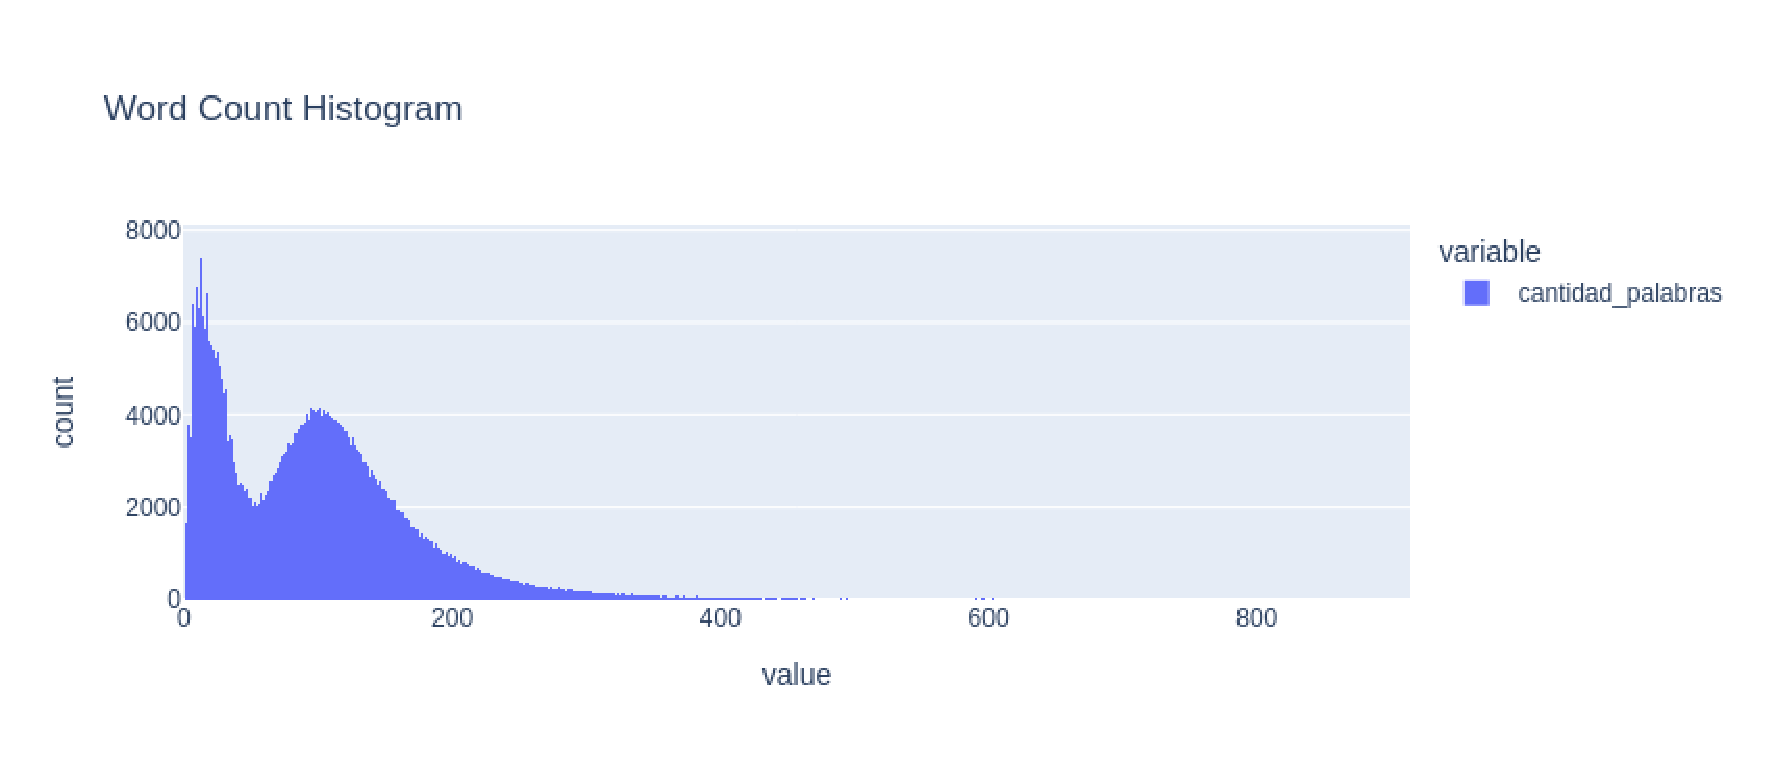
\includegraphics[width=\textwidth]{imgs/histograma.eps}
    \caption{Histogram of Word Count $l_w$ in Corpus $D^T$}
    \label{fig:histogramalw}
\end{figure}

\begin{figure}[!t]
    \centering
    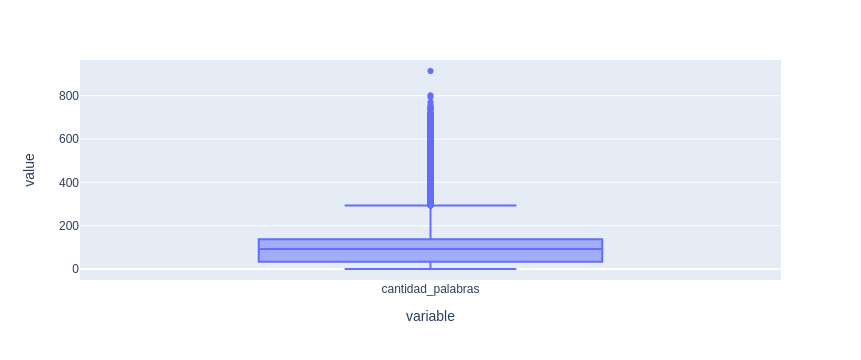
\includegraphics[width=\textwidth]{imgs/boxplot.png}
    \caption{Box Plot of Word Count $l_w$ in Corpus $D^T$}
    \label{fig:boxplotlw}
\end{figure}

\begin{figure}[!t]
    \centering
    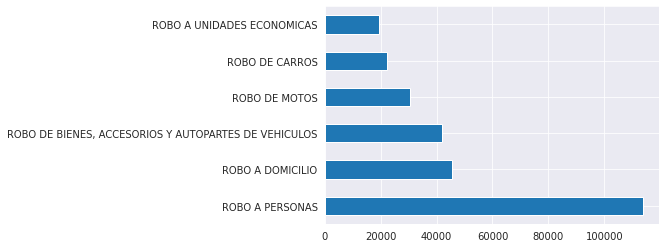
\includegraphics[width=\textwidth]{imgs/categorias.png}
    \caption{Text Categories of Dataset $D^T$}
    \label{fig:categorias}
\end{figure}

\begin{table}[!t]
% increase table row spacing, adjust to taste
\renewcommand{\arraystretch}{1.3}
% if using array.sty, it might be a good idea to tweak the value of
% \extrarowheight as needed to properly center the text within the cells
\caption{Statistical Values of the Dataset}
\label{tab: metricasorig}
\centering
% Some packages, such as MDW tools, offer better commands for making tables
% than the plain LaTeX2e tabular which is used here.
\begin{tabular}{c c}
\hline
\textbf{Metric} & \textbf{Value} \\
\hline
Count &    \numprint{671146} \\ %count
Mean     &   \numprint{98.34} \\ %mean
Std      &   \numprint{77.38} \\ %std
Min      &    \numprint{0} \\ %min
25\%      &   \numprint{33.00} \\
50\%      &   \numprint{92.00} \\
75\%      &  \numprint{137.00} \\
Max      &  \numprint{914.00} \\
\hline
\end{tabular}
\end{table}

\subsubsection{Organization of the dataset into training, validation, and testing subsets}

To train the model, it is necessary to split the dataset $D^T$ into
training subsets $D^T_{train}$ (\numprint{273336} records), validation
$D^T_{valid}$ (\numprint{68333} records), and testing $D^T_{test}$
(\numprint{90000} records). The subsets are obtained by randomly
selecting examples from the dataset $D^T$. The validation dataset was
obtained by splitting the training dataset into 80\%, 20\%. Thus, the
model training uses the number of examples presented in Table
\ref{tab:datasplit}.

\begin{table}[!t]
% increase table row spacing, adjust to taste
\renewcommand{\arraystretch}{1.3}
% if using array.sty, it might be a good idea to tweak the value of
% \extrarowheight as needed to properly center the text within the cells
\caption{Generation of Training, Validation, and Testing Datasets}
\label{tab:datasplit}
\centering
% Some packages, such as MDW tools, offer better commands for making tables
% than the plain LaTeX2e tabular which is used here.
\begin{tabular}{ccc}
\hline
Dataset Type & Records & \%\\
\hline
$D_{train}^T$ & \numprint{273336} & \numprint{63.32}\%\\
$D_{valid}^T$ & \numprint{68333} & \numprint{15.83}\%\\
$D_{test}^T$ & \numprint{90000} & \numprint{20.85}\%\\
\hline
\end{tabular}
\end{table}

Each dataset consists of the text corresponding to the narrative of
the event and a numerical label that is an integer from 0 to 5,
corresponding to each of the labels. Although the prepared dataset has
the quantities shown, for this first stage of model training, a subset
of data from each of the datasets was used due to hardware constraints
for training the model.

\subsection{Expanded Taxonomy (\(D_{\kappa=11}\)): Validated Crime
  Categories}
\label{sec:expand-taxon-d_validados}
Para el entrenamiento del modelo de \emph{delitos validados} se
realiza la generación de un dataset que integra los relatos del parte
de la policía nacional así como los registros del SIAF. De esta manera
se entrena al modelo con textos diferentes para cada Noticia del
Delito NDD. El dataset obtenido tiene un total de \numprint{1109335}
registros con 6 variables: NDD, Presunto Delito, Relato, delitos
seguimiento y delitos validados.

\begin{enumerate}
\item Lectura de registros de \printInicialesComision\, de 2014 a 2022
  donde Tipo Penal es Robo con las columnas NDD, Tipo Delito PJ,
  delitos seguimiento y delitos validados i.e.
  $\mathbb{D}_{735045 \times 4}^A$
        \item Obtención de relatos fiscalía y policía
          $\forall NDD_i \in \mathbb{D}_{735045\times4}^{A}$ desde la
          base de relatos $\mathbb{D}^{FGE\cup PN\cup CE}$:
          $\mathbb{D}_{725079 \times 8}^B$
        \item Se excluyen tipos penales diferentes de robo i.e. $\mathbb{D}_{723435 \times 8}^{B'} \subset \mathbb{D}_{725079 \times 8}^B$
        \item Se realiza el inner join segun los números de Noticia
          del Delito: \\
          $\mathbb{D}^{robos}_{723435\times 11} = \mathbb{D}_{735045
            \times 4}^A \bowtie_\theta \mathbb{D}_{723435 \times
            8}^{B'} $
        \item Formateo de relato: texto a minúsculas y retirar
          caracteres que no sean letras o números.
        \item Integrar la columna $relato_{pn}$ y $relato_{fge}$ en
          una sola columna de relato y conservando las columnas de
          NDD, Presunto Delito, Relato, delitos seguimiento y delitos
          validados i.e.
          $\mathbb{D}^{robos}_{1446870 \times 5} =
          \mathbb{D}^{robos_{pn}}_{723435\times 5} \cup
          \mathbb{D}^{robos_{fge}}_{723435\times 5}$
        \item Ordenar ascendente según valor de NDD a $\mathbb{D}^{robos}_{1446870 \times 5}$
        \item Analizar la estadística de la cantidad de palabras de
          los relatos de policía y fiscalía. Se conserva los relatos
          tales que: $50 \leq len(relato_i) \leq 400$. Pues, límite
          superior (\emph{upper fence}) del $q_3$ del relato de
          policía es $\numprint{389.5}$
          i.e. $\mathbb{D}^{robos}_{(1140728 \times 6)}$
          % \item Las columnas RelatoPolicia y RelatoFiscalia se
          %   concatenan y forman una sola columna denominada
          %   \emph{relato}
        \item Corregir etiquetas de delitos seguimiento: se sustituye
          las letras tildadas por sus equivalentes sin tilde
          e.g. económicas $\rightarrow$ economicas
        \item Delitos validados presenta un total de 48 categorías que
          no pertenecen a las 14 aceptadas. Por esta razón se: a)
          conserva aquellas con la etiqueta \say{OTROS ROBOS} y
          aquellas que no pertenezcan a las 14 aceptadas son
          descartadas, b) las categorías de \say{ROBO A INSTITUCIONES
            DE SALUD}, \say{ROBO EN EJES VIALES O CARRETERAS}, y
          \say{ROBO A ENTIDADES FINANCIERAS} se renombran como
          \say{OTROS ROBOS}. Se obtiene, entonces,
          $\mathbb{D}^{robos}_{(1109335 \times 6)}$ con las categorías
          definidas en Tabla \ref{tab:listofRobberiesValidados}.
        \item Las filas del dataset se orden aleatoriamente
        % \item Se salva los datos en sql:
        %     \begin{lstlisting}[language=Python]
        %         from src.utils import save_df_in_sql
        %         save_df_in_sql(dataf=dataset_out,name_table='dataset_RobosDesagregation06122023')
        %     \end{lstlisting}
    \end{enumerate}

\textbf{Notación:}\\
$\bowtie_\theta$: Inner Join donde $\theta:\mathbb{D}^A.NDD=\mathbb{D}^B.NDD$ 


La Tabla \ref{tab:GeneracionDataset} presenta las cantidades de
registro según categoría de \emph{delitos validados} obtenidas en la
generación del dataset. Se puede obsevar que la categoría de \emph{SIN
  INFORMACION} de \emph{delitos seguimiento} corresponde a categorías
diferentes a las 6 que se usaron en el modelo \emph{delitos
  seguimiento}. También se debe observar que la categoría \emph{OTROS
  ROBOS} será ahora predicha por el modelo.

\begin{table}[htbp]
        \centering
        \caption{Categorías de Delitos Validados y Seguimiento en el Dataset}
        \label{tab:GeneracionDataset}
        \scriptsize
        \begin{tabularx}{\textwidth}{p{0.4\textwidth}p{0.4\textwidth}X}
            \toprule
            delitos\_seguimiento & delitos\_validados & Total \\ \hline
            ROBO A DOMICILIO & ROBO A DOMICILIO & 172264 \\
            ROBO A PERSONAS & ROBO A PERSONAS & 421497 \\ ROBO A UNIDADES ECONOMICAS & ROBO A UNIDADES ECONOMICAS & 74088 \\ 
            ROBO DE BIENES, ACCESORIOS Y AUTOPARTES DE VEHICULOS & ROBO DE BIENES, ACCESORIOS Y AUTOPARTES DE VEHICULOS & 154546 \\
            ROBO DE CARROS & ROBO DE CARROS & 90038 \\ 
            ROBO DE MOTOS & ROBO DE MOTOS & 119128 \\ \hline 
            \multirow{4}{*}{SIN INFORMACION}  & OTROS ROBOS & 43468 \\ 
            {} & ROBO A EMBARCACIONES DE ESPACIOS ACUATICOS & 9407 \\ 
            {} & ROBO A ESTABLECIMIENTOS DE COLECTIVOS U ORGANIZACIONES SOCIALES & 3087 \\ 
            {} & ROBO A INSTITUCIONES EDUCATIVAS & 17252 \\
            {} & ROBO EN INSTITUCIONES PUBLICAS &  4560 \\ \hline
            \multicolumn{2}{c}{Total} & \numprint{1109335} \\
            \bottomrule
        \end{tabularx}
        % \caption{Categorías de Delitos Validados y Seguimiento en el Dataset}
        % \label{tab:groupbycategorias}
    \end{table}

\subsubsection{Organización de Dataset para Entrenamiento, Validación y Test}

Una de las técnicas más comunes para el entremaniento de modelos de
aprendizaje profundo (\emph{deeplearning}) consiste en separar el
dataset en subconjuntos de entrenamiento, validación y prueba. La idea
de esto es poder probar la capacidad de generación del modelo
entrenado. Recuérdese, también que la técnica de \emph{Fine Tuning}
permite reducir el número de ejemplos con los que se entrena el
modelo, reduciendo de los millones de ejemplos iniciales con los que
son entrenados los modelos a utilizar datasets con cientos de miles de
datos, obteniendo resultados adecuados.

\begin{enumerate}
        \item Los datos se organizan de la siguiente manera:
        \begin{itemize}
            \item Entrenamiento: \numprint{807468} $\approx$ 72\%
            \item Validación: \numprint{201867} $\approx$ 18\%
            \item Test: \numprint{100000} $\approx$ 10\%
        \end{itemize}
        \item El dataset se separa en dos subconjuntos dependiendo si las etiquetas corresponden a delitos seguimiento o delitos validados
        \item Se conserva únicamente el relato y la etiqueta (i.e. delitos\_validados) que se renombra como \emph{labels}.
        \item Los datos se guardan en la base de datos de \emph{Machine Learning}:
            % \scriptsize
            % \begin{lstlisting}[language=Python]
            %     from src.utils import save_df_in_sql
            %     save_df_in_sql(
            %          dataf=train_delitos_validados_huggingface,
            %         database="machinelearning",
            %         name_table="train_delitos_validados_hf",
            %     )            
            %     save_df_in_sql(
            %         dataf=valid_delitos_validados_huggingface,
            %         database="machinelearning",
            %         name_table="valid_delitos_validados_hf",
            %     )
            %     save_df_in_sql(
            %         dataf=test_delitos_validados_huggingface,
            %         database="machinelearning",
            %         name_table="test_delitos_validados_hf",
            %     )
            % \end{lstlisting}
        
    \end{enumerate}

\section{Methodology}\label{chap:metodos}
\subsection{Problem Formulation}

Text classification consists of obtaining a function $f$ that maps a
Dataset $D$, composed of text sequences
$X_i \in D=\{X_1, X_2, \dots, X_N\}$ to $k$ categories. Each document
$X_i$ is composed of $s$ sentences and each sentence of $w_s$ words,
which in turn have $l_w$ letters\footnote{We consider to use the
  notation presented in \cite{Kowsari2019}}. The classification
operation is thus represented by Equation \eqref{eq:clasificacion}.

\begin{equation}\label{eq:clasificacion}
    f: D \longrightarrow \mathbb{Z}^k
\end{equation}

However, for the model to be processed by a computing system or AI,
the different documents $X_i$ must be represented (\emph{encoding})
appropriately, so that the textual information is represented
numerically. Therefore, the four traditional stages of a text
classification system, such as: feature extraction, dimensionality
reduction, classification, and evaluation, have been simplified thanks
to the characteristics of the DL approach that allow a automatic
feature extraction as explained in \ref{sec:arch-fond-bert}.

% The use of Recurrent Neural Networks (RNN) allows for automatic
% feature extraction, while the autoencoder architecture, in its
% \emph{encoding} stage, allows for information representation and, if
% required, dimensionality reduction.
% ==================== original ====================
% The problem consists of classifying crime report narratives into
% specified robbery subcategories. As represented in Equation
% \ref{eq:clasificacion}, this is a supervised text classification
% task. To adapt the pre-trained `distilbert-base-multilingual-cased`
% model, both transfer learning (TL) and fine-tuning (FT) were employed
% to specialize the model for this domain-specific task. The
% classification task requires converting text sequences into numerical
% representations through a multi-step process. Let
% $\Tokenize: \mathcal{X} \rightarrow \mathbb{Z}^\lambda$ be the
% tokenization function that maps text sequences to token IDs, where
% $\mathcal{X}$ is the text space and $\lambda$ is the maximum sequence
% length. For each input sequence $X_i \in D^T_N$, BERT's tokenizer
% produces:

% \begin{equation}
%     (\boldsymbol{\nu}_i, \boldsymbol{\tau}_i) = \Tokenize(X_i)
% \end{equation}

% where $\boldsymbol{\nu}_i \in \mathbb{Z}^\lambda$ are the token IDs
% and $\boldsymbol{\tau}_i \in \{0,1\}^\lambda$ is the attention
% mask. These are then processed by BERT's embedding layer to generate
% contextual representations:

% \begin{equation}
%   \mathbf{H} = \text{BERT}((\boldsymbol{\nu}_i, \boldsymbol{\tau}_i)) \in \mathbb{R}^{\lambda \times d}
% \end{equation}

% where $d$ is the hidden dimension size. The classification head then
% maps the [CLS] token representation to label space:

% \begin{equation}
%     \hat{\boldsymbol{y}}_i = f(\mathbf{h}_{[\text{CLS}]}) \in \mathbb{R}^k
% \end{equation}

% To
% convert the text sequences into a numerical representation,
% tokenization of the examples $D^T$ is necessary. Let $\Tokenization$
% be a function that allows obtaining the tokenization of text
% sequences, then Equation \ref{eq:encoding} represents the encoding of
% the target dataset $D^T$.

% \begin{equation}\label{eq:encoding}
%     \mathbf{embeddings} = \Tokenization(D^T)
% \end{equation}

% The operation indicated in \eqref{eq:encoding} converts the text
% sequences into feature vectors
% $\boldsymbol{\nu} \in \mathbb{Z}^{\lambda}$ and
% $\boldsymbol{\tau} \in \mathbb{Z}^\lambda$; which represent the
% numerical encoding and the attention mask, respectively. $\lambda$ is
% the maximum sequence length of the text. If $X_i \in D^T_{N}$ is a
% text sequence of length $\lambda$ and $N$ is the number of records in
% $D^T$, then \eqref{eq:clasificacion} can be rewritten as

% \begin{equation}\label{eq: tensorflowin}
%     \dot{f}: \mathbb{Z}^{(N,\lambda,2)} \longrightarrow \mathbb{Z}^k
% \end{equation}

% Where the classification prediction is also a one-hot vector
% $\boldsymbol{y}_i$.


The problem consists of classifying crime report narratives into
specified robbery subcategories. To adapt the pre-trained
\texttt{distilbert-base-multilingual-cased} model, both transfer
learning (TL) and fine-tuning (FT) were employed to specialize the
model for this domain-specific task.

The classification process involves converting text sequences into
numerical representations through several stages. The processing
pipeline consists of:

\begin{enumerate}
    \item \textbf{Tokenization}: Converting raw text to token IDs
    \item \textbf{Embedding}: Mapping tokens to vector representations
    \item \textbf{Contextual Encoding}: Generating sequence-aware representations
    \item \textbf{Classification}: Predicting labels from [CLS] token
\end{enumerate}

Which can be written as:

\begin{equation*}
\text{Raw Text} \xrightarrow{\Tokenize} \text{Token IDs} \xrightarrow{\text{Embedding}} \text{Vectors} \xrightarrow{\bertmodel} \text{Contextual Representations} \xrightarrow{\text{Head}} \text{Predictions}
\end{equation*}

Let $\Tokenize: \mathcal{X} \rightarrow \mathbb{Z}^\lambda$ be the
tokenization function that maps text sequences to token IDs, where
$\mathcal{X}$ is the text space and $\lambda$ is the maximum sequence
length. For each input sequence $X_i \in D^T_N$, the tokenizer
produces:

\begin{equation}\label{eq:tokenization}
    (\boldsymbol{\nu}_i, \boldsymbol{\tau}_i) = \Tokenize(X_i)
\end{equation}

where:
\begin{itemize}
    \item $\boldsymbol{\nu}_i \in \mathbb{Z}^\lambda$ are the token IDs
    \item $\boldsymbol{\tau}_i \in \{0,1\}^\lambda$ is the attention mask
\end{itemize}

These token IDs are then passed through the embedding layer:

\begin{equation}\label{eq:embedding}
    \mathbf{E} = \text{Embedding}(\boldsymbol{\nu}_i) \in \mathbb{R}^{\lambda \times d}
\end{equation}

where $d$ is the embedding dimension. The complete \bertmodel{} model
processes these embeddings to produce contextual representations:

\begin{equation}\label{eq:encoding}
    \mathbf{H} = \bertmodel{}(\mathbf{E}, \boldsymbol{\tau}_i) \in \mathbb{R}^{\lambda \times d}
\end{equation}

The classification head uses the [CLS] token representation
($\mathbf{h}_{[\text{CLS}]} \in \mathbb{R}^d$) to predict the label:

\begin{equation}\label{eq:classification}
  \hat{\boldsymbol{y}}_i = \text{softmax}(\mathbf{W}\mathbf{h}_{[\text{CLS}]} + \mathbf{b}) \in \mathbb{R}^k
\end{equation}

where:
\begin{itemize}
  \item $\mathbf{W} \in \mathbb{R}^{k \times d}$ is the classification weight matrix
  \item $\mathbf{b} \in \mathbb{R}^k$ is the bias term
  \item $k$ is the number of target categories
\end{itemize}


Consequently, for a text sequence $X_i \in D^T_{\kappa, N}$ of length
$\lambda$ where $N$ is the number of records, and $\kappa$ the number
of categories, in the target dataset $D^T$, the classification
function from Equation \eqref{eq:clasificacion} can be formally
expressed as:

\begin{equation}\label{eq:tensor_mapping}
    f: \mathbb{Z}^{N \times \lambda \times 2} \to \mathbb{R}^k
\end{equation}

where:
\begin{itemize}
    \item $\mathbb{Z}^{N \times \lambda \times 2}$ represents the batched input tensor containing:
    \begin{itemize}
        \item Token IDs $\boldsymbol{\nu}_i \in \mathbb{Z}^\lambda$
        \item Attention masks $\boldsymbol{\tau}_i \in \{0,1\}^\lambda$
    \end{itemize}
    \item $\mathbb{R}^k$ denotes the probability distribution over $k$ categories (with softmax activation)
    \item The dot notation ($\dot{f}$) is replaced with standard function notation for clarity
\end{itemize}


% Consequently, If $X_i \in D^T_{N}$ is a
% text sequence of length $\lambda$ and $N$ is the number of records in
% $D^T$, then \eqref{eq:clasificacion} can be rewritten as

% \begin{equation}\label{eq: tensorflowin}
%     \dot{f}: \mathbb{Z}^{(N,\lambda,2)} \longrightarrow \mathbb{Z}^k
% \end{equation}
  
The TL operation defined according to \textcite{falconi2020transfer}
is stated as a functional operation that aims to save the weights of
the model $\boldsymbol{W}^S$ pre-trained on an original dataset $D^S$
in a similar domain and place at the output of said model layers that
adapt the encoding of the trained model and adjust it to the target
task, in a target dataset $D^T$; where the number of examples in the
original dataset is significantly greater than that of the target
dataset: $\Lambda(D^S) \ggg \Lambda(D^T)$ and $\Lambda$ returns the
size of records in the dataset. Therefore, the following definition of
TL given in \cite{falconi2020transfer} is considered:

\begin{definition}
  Given an original domain $\mathcal{D}^{S}$ with an original learning
  task $\mathcal{T}^{S}$, a target domain $\mathcal{D}^{T}$, with a
  target task $\mathcal{T}^{T}$, the TL operation seeks to improve the
  learning of a prediction function $\ypredtarget(\cdot)$ in
  $\mathcal{D}^{T}$ using the knowledge acquired in
  $\ypredsource(\cdot)$ in $\mathcal{T}^{S}$, through $\phi^S$; where
  $\mathcal{D}^{S} \neq \mathcal{D}^{T}$ or
  $\mathcal{T}^{S} \neq \mathcal{T}^{T}$.
\end{definition}

Considering the mentioned definition of TL, \eqref{eq:Transfer2}
represents the TL operation applied to the text classification
problem, starting from a pre-trained natural language model; where $L$
is the number of layers of the pre-trained model.

\begin{equation}
  \mathbb{T_{L}} \left< \ypredsource(\mathcal{D}^{S}), \mathcal{D}^{T}  \right> = \ConvNetOut \left(\ypredsource(\mathcal{D}^{T}) \Bigr\rvert_{0}^{L} \right)
    \label{eq:Transfer2}
\end{equation}

Consequently, the prediction generation is represented by Equation
\eqref{eq:Transfer3}
\begin{equation}
    \mathcal{Y}^{T} = \mathbb{T_{L}} \left< \ypredsource(D^{S}), \mathcal{D}^{T} \right> = \ypredtarget(D^T) 
    \label{eq:Transfer3}
\end{equation}



\subsection{Phase 1: Baseline Transfer Learning}\label{sec:phase-1:-baseline}
Transfer learning, as indicated by Equations \ref{eq:Transfer2} and
\ref{eq:Transfer3}, allows adjusting the original training
$\ypredsource(\cdot)$ to adapt it to the target task
$\ypredtarget(\cdot)$. For this, a series of layers represented by
functional operations $\mathcal{A}$ are used, which will allow the
model to be adjusted. During training, the weights of the pre-trained
\emph{\modelohuggingface} model $\ypredsource(\cdot)$, denoted as
$\mathcal{W}^S$, are not modified and are used as a \emph{feature
  extractor}. The pre-trained model contains a total of
$\mathcal{W}^S = \numprint{134734080}$ parameters, which will not be
trained. The output of the pre-trained model is a tensor
$\mathbb{R}^{(N \times 300 \times 768)}$. Using Global Max Pooling
$GMP$, the tensor is transformed into one of dimension
$\mathbb{R}^{(N \times 768)}$. The application of the operations
$\mathcal{A}$, described in Equation \ref{eq:finetuning}, generates a
weight matrix $\mathcal{W}^T$ corresponding to the different layers
added for this purpose. These layers are operationally represented in
Equation \ref{eq:finetuning} and consist of: Batch Normalization $BN$,
Fully Connected Layer with 512 neurons $FC_{512}$, Drop Out of 0.1
$Dro_{0.1}$, 2 sets of Fully Connected Layers with 128 neurons
$FC_{128}$ and Drop Out of 0.1 $Dro_{0.1}$, and finally an output
layer with 6 neurons $Fc_{6}$. Consequently, it is not necessary to
train the entire final model $\mathcal{W}^S+\mathcal{W}^T$, but only
the output layers $\mathcal{W}^T$, which corresponds to
$\mathcal{W}^T = \numprint{478214}$.

\begin{IEEEeqnarray}{lCr}\label{eq:finetuning}
    \mathcal{A} = FC_{6} \circ Dro_{0.1} \circ FC_{128}  \circ Dro_{0.1} \circ FC_{128} \\ 
    \circ Dro_{0.1} \circ FC_{512} \circ BN \circ GMP \nonumber
\end{IEEEeqnarray}

\subsubsection{Model Training}\label{sec:phase1-model-training}
The model training consists of using \emph{TL} to fine-tune a
pre-trained model for the desired classification task. In this way, it
will be possible to predict the category to which a robbery text
belongs, choosing among the 6 previously indicated categories (Figure
\ref{fig:categorias}). The pre-trained model used is
\emph{\modelohuggingface}. Although the pre-trained model and the
generated dataset were loaded using the HuggingFace
\emph{transformers} API, the model training was performed in
\emph{Tensorflow}. The steps followed during training are as follows:

\begin{enumerate}
    \item Loading of the datasets $D^T_{train}$, $D^T_{valid}$, $D^T_{test}$
    \item Tokenization of the datasets
    \item Resampling of the datasets (due to hardware limitations)
    \item Obtaining the input tensors, mask, and classification
      tensors in one-hot encoding.
    \item Loading the pre-trained model $\ypredsource(\cdot)$
    \item The fine-tuning model is obtained by applying $\mathcal{A}$: $y^T = \ypredtarget(\mathbf{\mathcal{X}}^T) =  \mathcal{A}(\ypredsource(\mathbf{\mathcal{X}}^T))$
    \item The model is compiled with the training parameters presented
      in Table \ref{tab:trainingParam}.
    \item Training is executed in Google Colab.
    \item Backup of the training weights.
\end{enumerate}

Tokenization allows converting the text into a tensor representation
that is used by the computer for training the Machine Learning
model. For the studied case, since the histogram of the number of
words per document indicates a maximum sequence length of
$\lambda = 300$ words, the mask and input tensors are of
$\mathbf{\mathcal{X}}^{N\times300}$; where $N$ is the number of
examples.

Due to hardware limitations used for training (Google Colab), the
examples were reduced to
$d^T_{train}:\numprint{20000} \subset D^T_{train}$,
$d^T_{valid}:\numprint{4000} \subset D^T_{valid}$,
$d^T_{test}:\numprint{4000} \subset D^T_{test}$.

\begin{table}[!t]
% increase table row spacing, adjust to taste
\renewcommand{\arraystretch}{1.3}
% if using array.sty, it might be a good idea to tweak the value of
% \extrarowheight as needed to properly center the text within the cells
\caption{Training Parameters}
\label{tab:trainingParam}
\centering
% Some packages, such as MDW tools, offer better commands for making tables
% than the plain LaTeX2e tabular which is used here.
\begin{tabular}{cc}
\hline
Parameter & Value\\
\hline
Loss & Categorical Cross Entropy\\
Metrics & Categorical Accuracy \\
Optimizer & Adam \\
Learning rate & $2 \times 10^{-4}$ \\
epochs & 10 \\
callback & 5 epochs \\
\hline
\end{tabular}
\end{table}

\subsection{Phase 2: Fine-Tuning on Dataset $D_{\kappa=6}$}
\label{sec:phase-2:-finetuningBert}
The TL technique uses the trained weights of a Deep Learning model on
another $\mathcal{D}^{S}$ with an original learning task
$\mathcal{T}^{S}$. Section \ref{sec:phase-1:-baseline} presented the
architecture used to adapt the original classification
$\mathcal{T}^{S}$ to obtain Model $\phi^T(\cdot)$ for classifying
\textbf{delito seguimiento} (follow-up crime) labels in robbery news
articles. As expressed in \eqref{eq:Transfer2}, the weights trained on
the original task $\mathcal{W}^S$ are not adapted in any way for the
new task $\mathcal{W}^T$. Consequently, Model $\phi^S(\cdot)$ is used
as a feature extractor. Section \ref{chap:resultados} shows that the
classifier's performance, trained via TL to predict follow-up crime
labels, achieved an average accuracy of 80\%.

According to \textcite{tunstall2022natural},
performing \emph{Fine Tuning} (FT) of all the model's original weights
allows adaptation of the hidden states during training to reduce loss
and thereby increase classifier performance in the new task
$\phi^T(\cdot)$. \textcite{falconi2020transfer} defines FT as the
process that improves the learning of a target function
$\mathcal{Y}^T = \ypredtarget(\mathcal{I}^T)$ in a target domain
$\mathcal{D}^T$ for a target task $\mathcal{T}^T$ by retraining $r$
layers of the original model
$\mathcal{Y}^S = \ypredsource(\mathcal{I}^S)$ with $L$ layers, trained
on an original domain $\mathcal{D}^S$ and original task
$\mathcal{T}^S$.

\begin{equation}
    \mathbb{F_{T}} \left< \ypredsource(\mathcal{D}^{S}), \mathcal{D}^{T} \right> = \ConvNetOut \left( \ypredsource \left (\ypredsource(\mathcal{D}^{T}) \Bigr\rvert_{0}^{\gamma -1} \right)\Bigr\rvert_{\gamma}^{L}\right) 
    % \gamma = L-r \nonumber
    \label{eq:finetuningLenin}
\end{equation}

Equation \eqref{eq:finetuningLenin} symbolically represents the FT
definition, where $\mathcal{A}$ denotes the FT process on the original
$L$-layer model, and $\gamma = L-r$ is the layer from which
fine-tuning starts. A special case is full model tuning: $r=L$ implies
$\gamma=0$, as recommended by \citeauthor{tunstall2022natural} in
\citetitle{tunstall2022natural}. While
\textcite{falconi2020transfer}'s definition allows tuning only some
layers, setting $r=L$ eliminates the need for additional output
layers, affecting only the neurons corresponding to the new
classes. Thus, following \textcite{tunstall2022natural}'s assertion
that tuning all hidden states improves performance, the FT operation
used is:


\begin{equation}\label{eq: finetuningTunstall}
    \mathbb{F_{T}} \left< \ypredsource(\mathcal{D}^{S}), \mathcal{D}^{T} \right> = \ConvNetOut \left(\ypredsource(\mathcal{D}^{T})\right)
\end{equation}

Here, omitting $\Bigr\rvert_{0}^{L}$ implies full model adjustment,
initializing weights with $\mathcal{W}^S$ values (i.e.,
$\mathcal{W}^S\rightarrow \mathcal{W}^T$). Additionally:

\begin{align}\label{eq:finetuningOut}
    \mathcal{A} = FC_{6}
\end{align}


To improve model learning on robbery complaint data and their relation
to follow-up crime labels used by the Comisión, the following steps
were taken, based on \textcite{tunstall2022natural}'s hypothesis that
FT improves classification over TL:

\begin{enumerate}
    \item Loading datasets $D^T_{train}$, $D^T_{valid}$, $D^T_{test}$
    \item Tokenizing datasets with a maximum sequence length of 300 using the \emph{distilbert-base-multilingual-cased} tokenizer
    \item Resampling datasets (due to hardware constraints): Training uses $|d_{train}^T| = \numprint{20000}$ samples, validation $|d_{valid}^T| = \numprint{4000}$, and testing $|d_{test}^T| = \numprint{4000}$.
    \item Generating input tensors, masks, and one-hot encoded classification tensors.
    \item Loading the pre-trained model $\ypredsource(\cdot)$
    \item Applying FT via \eqref{eq: finetuningTunstall}
    \item Compiling the model with parameters in Table \ref{tab:trainingParam2}
    \item Training on Google Colab
    \item Backing up trained weights
\end{enumerate}

\begin{table}
    \caption{Improved Model Training Parameters}
    \label{tab:trainingParam2}
    \centering
    \begin{tabular}{cc}
    \hline
    Parameter & Value\\
    \hline
     Loss & Sparse Categorical Cross Entropy\\
    Metrics & Sparse Categorical Accuracy \\
    Optimizer & Adam \\
    Learning rate & $5 \times 10^{-5}$ \\
    epochs & 10 \\
    callback & No \\
    \hline
    \end{tabular}
  \end{table}

  
\subsection{Phase 3: Scaling to Dataset $D_{\kappa=11}$}
\label{sec:phase-3:-scaling-fullmodel}

The results in Section \ref{sec:phase-2:-finetuningBert} show that FT
improves classifier performance. Building on this, we now automate the
prediction of \emph{delitos validados} (validated crimes) labels
proposed by the \printInicialesComision, which include more robbery
subcategories. The new categories are presented in Table
\ref{tab:listofRobberiesValidados}. A total of 11 categories were
established. Among those categories, the previous 6 categories used
are present. % improve this writing

This section describes the methodology and results for improving
robbery subcategory prediction under \emph{delitos validados}. A new
dataset was created using police reports and Fiscalía General del
Estado (FGE) records from SIAF to increase data variability. Textual
similarity analysis at the embedding level between police and SIAF
reports was performed. Training utilized \emph{Tensor Processing
  Units} (TPUs) to handle increased categories and improve
precision. Dataset generation is described in Section
\ref{sec:expand-taxon-d_validados}.

\subsubsection{Validated Crimes Categories}

Per agreements between Fiscalía and INEC, Table
\ref{tab:listofRobberiesValidados} defines the validated crime
categories. The \say{OTROS ROBOS} (Other Robberies) category includes:
ROBO A INSTITUCIONES DE SALUD (Healthcare Institution Robbery), ROBO
EN EJES VIALES O CARRETERAS (Road/Highway Robbery), and ROBO A
ENTIDADES FINANCIERAS (Financial Institution Robbery).

%     \begin{table}[htbp]
%     \centering
%     \scriptsize
%     \begin{tabularx}{\textwidth}{|c|X|c|X|}
%         \hline
%         \textbf{Idx} & \textbf{Robbery Type} & \textbf{idx} & \textbf{Robbery Type} \\
%         \hline
%         0 & ROBO A INSTITUCIONES EDUCATIVAS\footnote{Educational Institution Robbery} & 6 & ROBO A UNIDADES ECONOMICAS\footnote{Economic Unit Robbery} \\
%         1 & ROBO DE MOTOS\footnote{Motorcycle Robbery} & 7 & ROBO A DOMICILIO\footnote{Home Robbery} \\
%         2 & ROBO EN INSTITUCIONES PUBLICAS\footnote{Public Institution Robbery} & 8 & ROBO DE BIENES, ACCESORIOS Y AUTOPARTES DE VEHICULOS\footnote{Vehicle Goods/Accessories Robbery} \\
%         3 & ROBO DE CARROS\footnote{Car Robbery} & 9 & ROBO A EMBARCACIONES DE ESPACIOS ACUATICOS\footnote{Watercraft Robbery} \\
%         4 & ROBO A ESTABLECIMIENTOS DE COLECTIVOS U ORGANIZACIONES SOCIALES\footnote{Collective/Organization Robbery} & 10 & OTROS ROBOS\footnote{Other Robberies} \\
%         5 & ROBO A PERSONAS\footnote{Person Robbery} & & \\
%         \hline
%     \end{tabularx}
%     \caption{Validated Crimes}
%     \label{tab:listofRobberiesValidados}
%   \end{table}

\begin{table}[htbp]
    \centering
    \scriptsize
    \begin{threeparttable}
    \caption{Validated Crimes}
    \label{tab:listofRobberiesValidados}
    \begin{tabularx}{\linewidth}{|c|X|c|X|}
        \hline
        \textbf{Idx} & \textbf{Robbery Type} & \textbf{Idx} & \textbf{Robbery Type} \\
        \hline
        0 & ROBO A INSTITUCIONES EDUCATIVAS\tnote{a} & 6 & ROBO A UNIDADES ECONOMICAS\tnote{f} \\
        1 & ROBO DE MOTOS\tnote{b} & 7 & ROBO A DOMICILIO\tnote{g} \\
        2 & ROBO EN INSTITUCIONES PUBLICAS\tnote{c} & 8 & ROBO DE BIENES, ACCESORIOS Y AUTOPARTES DE VEHICULOS\tnote{h} \\
        3 & ROBO DE CARROS\tnote{d} & 9 & ROBO A EMBARCACIONES DE ESPACIOS ACUATICOS\tnote{i} \\
        4 & ROBO A ESTABLECIMIENTOS DE COLECTIVOS U ORGANIZACIONES SOCIALES\tnote{e} & 10 & OTROS ROBOS\tnote{j} \\
        5 & ROBO A PERSONAS\tnote{k} & & \\
        \hline
    \end{tabularx}
    \begin{tablenotes}[flushleft]
        \item[a] Educational Institution Robbery
        \item[b] Motorcycle Robbery
        \item[c] Public Institution Robbery
        \item[d] Car Robbery
        \item[e] Collective/Organization Robbery
        \item[f] Economic Unit Robbery
        \item[g] Home Robbery
        \item[h] Vehicle Goods/Accessories Robbery
        \item[i] Watercraft Robbery
        \item[j] Other Robberies
        \item[k] Person Robbery
    \end{tablenotes}
    \end{threeparttable}
\end{table}




\subsubsection{Problem Formulation}
We aim to train an ML model to approximate a parametric function
$f_\theta$ mapping input $\mathbf{x}_i \in \mathbf{\mathcal{X}}$ to
category $k_j \in \mathcal{Y}$, where
$\mathcal{Y} \in \mathbb{R}^{11}$ (see Table \ref{tab:
  metricasorig}). Text is tokenized using the pre-trained model:

\begin{equation}\label{eq:clasificacion}
  f_\theta: \mathbf{\mathcal{X}} \longrightarrow \mathbf{\mathcal{Y}}
\end{equation}

For a narrative $relato_i \in \mathbb{D}^{PN}$ (or
$\mathbb{D}^{FGE}$), the tokenization step produces:

\begin{equation}
(\boldsymbol{\nu}_i, \boldsymbol{\tau}_i) = \Tokenize(relato_i)
\end{equation}

where the notation follows Equations \ref{eq:tokenization}-\ref{eq:encoding} in Section \ref{chap:metodos}. The final classification assigns $relato_i$ to category $k_j$ from Table \ref{tab: metricasorig}.

For the rest of the section consider the following nomenclature:

\begin{itemize}
\item $\mathbb{D}^{PN}$: Dataset from Policía Nacional narratives
\item $\mathbb{D}^{FGE}$: Dataset from Fiscalía General del Estado narratives 
\end{itemize}

\subsubsection{Text Similarity Analysis}
Due to computational limits (over 700K records), a sample of 6,000 reports was analyzed. Figure \ref{fig:metodologiaSimilitudTexto} outlines the methodology:

\begin{enumerate}
    \item Compare document similarity between $\mathbb{D}^{PN}$ and $\mathbb{D}^{FGE}$ samples
    \item Use two techniques: word2vec and Transformers
    \item Compute cosine similarity between embeddings:
\end{enumerate}

\begin{equation}\label{eq:cosinesimilarity}         
        \cos(\Gamma(x_i^{PN}), \Gamma(x_i^{FGE})) = \frac{\Gamma(x_i^{PN})\cdot\Gamma(x_i^{FGE})}{\|\Gamma(x_i^{PN})\|\|\Gamma(x_i^{FGE})\|}
\end{equation}
where $x_i^{PN} \in \mathbb{D}^{PN}$ and $x_i^{FGE} \in \mathbb{D}^{FGE}$

\paragraph{Methodology}
\begin{figure}
    \centering
    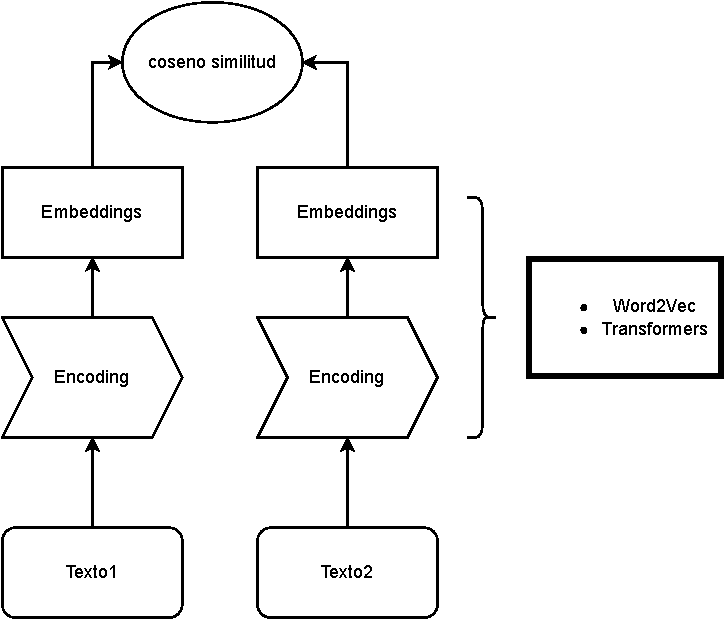
\includegraphics[scale=.75]{imgs/CosenoSimilitud.drawio.pdf}
    \caption{Text Similarity Calculation Methodology}
    \label{fig:metodologiaSimilitudTexto}
\end{figure}

Steps:
\begin{enumerate}
    \item Calculate sample size $n=6000$ (90\% confidence, 1.06\% margin of error)
    \item Randomly select $n$ reports with $E(w)\geq50$ words
    \item Generate embeddings using word2vec and Transformers
    \item Compute cosine similarity via \eqref{eq:cosinesimilarity}
    \item Statistically compare results
    \item Compare classifier predictions on police vs. fiscal reports
\end{enumerate}

\paragraph{Sample Size Calculation}
\begin{equation*}
        n =\frac{z^2p(1-p) }{\epsilon^2N+z^2p(1-p)}N
\end{equation*}

Where:\\
$N = \numprint{785513}$ \\
$p = \numprint{0.5}$ \\
$z = \numprint{1.65}$  \\
$\epsilon = \numprint{1.06}\%$ \\
$n = \numprint{6012} \approx \numprint{6000}$

The results of the sample size calculation with the obtained variables
can be consulted online at the
\href{https://www.calculator.net/sample-size-calculator.html?type=1&cl=90&ci=1.06&pp=50&ps=785513&x=Calculate}{Sample
  Calculator Link}. Consequently, a sample of \numprint{6000} records
is required to present results with \numprint{90}\% confidence from a
total of \numprint{785513}.

\paragraph{Obtaining Embeddings}  
For computational systems to process text, it is necessary to convert
the text into a numerical vector representation (i.e.,
\emph{embedding}). Equation \eqref{eq:encoding} represents this
process. To ensure objectivity in this experiment, two fundamentally
different techniques are proposed: \emph{word2vec} and
\emph{transformers}.

\begin{itemize}
\item \textbf{Word2vec}: A natural language processing technique that
  enables vector representation of words in a corpus. It uses a
  3-layer neural network trained on the corpus. Words that share
  similar contexts will have vectors close to each other in the vector
  space. Thus, Word2vec allows representing words as numerical vectors
  in a low-dimensional space.

\item \textbf{Transformers}: Transformers are deep learning models
  that use attention mechanisms to capture relationships between words
  in a text. To obtain embeddings with transformers, the hidden states
  from the final layer of the model are typically used (or pooled), as
  these encode contextualized semantic and syntactic features. In this
  specific case, the \modelohuggingface model has been utilized.
\end{itemize}

\paragraph{Text Similarity Results}
Table \ref{tab:resultadosCosSim} presents the statistical results
obtained from computing the cosine similarity of vector
representations of police reports (relatos de policía) and Fiscalía
General del Estado (FGE) reports using two different techniques
(word2vec and transformers). It can be observed that the mean
similarity exceeds 95\%.

\begin{table}[htbp]
\caption{Document Similarity Results}
\label{tab:resultadosCosSim}
\centering
    \begin{tabular}{l l l}   
    \toprule
     & word2vec & bert-transformer \\ \hline
    count & \numprint{6000} & \numprint{6000} \\ 
    mean & \numprint{0.957418} & \numprint{0.987899} \\
    std & \numprint{0.073233} & \numprint{0.023865} \\
    min & \numprint{0.310206} & \numprint{0.780015} \\
    25\% & \numprint{0.961602} & \numprint{0.990691} \\
    50\% & \numprint{0.975714} & \numprint{0.995396} \\
    75\% & \numprint{0.984985} & \numprint{0.997255} \\
    max & 1 & 1 \\
    \bottomrule
    \end{tabular}
    
\end{table}

\paragraph{Text similarity through Label Prediction with the Phase 2 Model}
Additionally, to analyze the similarity between police reports and FGE
reports, predictions were made using a pre-trained \emph{delitos
  seguimiento} model independently on both report sets according to
\eqref{eq:prediccionRelatoPolicia} and
\eqref{eq:prediccionRelatoFGE}. The classifier's performance
evaluation indicates that the model adequately generalizes text
comprehension and is not affected by the report's origin. Thus,
transformer-based models acquire knowledge of text semantics, and
their results are coherent. This disproves assumptions that model
performance would degrade depending on whether the input is a police
report (parte policial) or an SIAF registry. Figure
\ref{fig:comparacionDelitosSeguimientoRelatos} shows that predicted
categories follow similar trends, with a minimal numerical difference:
the global disparity between predictions on police and FGE reports is
\numprint{0.16}\%.

\begin{equation}\label{eq:prediccionRelatoPolicia}
    y^{PN} = f_\theta(\mathbf{\mathcal{X}}^{PN})
\end{equation}

\begin{equation}\label{eq:prediccionRelatoFGE}
    y^{FGE} = f_\theta(\mathbf{\mathcal{X}}^{FGE})
\end{equation}

\begin{figure}[h!]
    \centering
    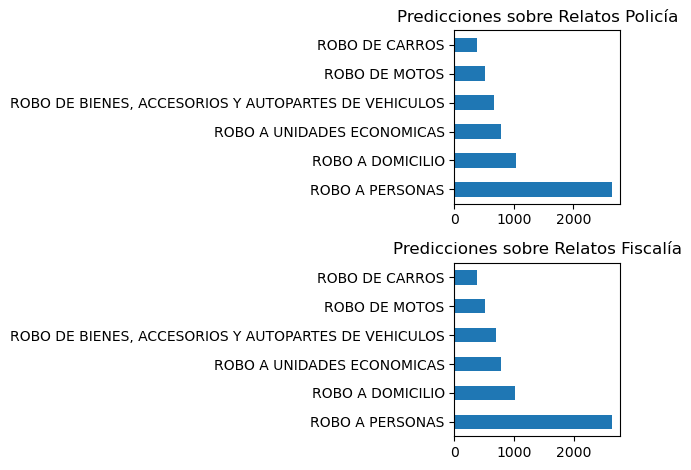
\includegraphics[width=\textwidth]{imgs/prediccionDelitosSeguimientoPoliciaVsFiscalia.png}
    \caption{Prediction comparison between police reports and FGE reports}
    \label{fig:comparacionDelitosSeguimientoRelatos}
\end{figure}

For full-data training, we leveraged TPU (Tensor Processing Unit)
hardware advantages. TPUs, designed by Google for machine learning
with neural networks (especially \emph{deep learning} frameworks like
\emph{TensorFlow} or \emph{PyTorch}), excel at parallelized complex
mathematical operations, high-speed memory bandwidth, and
mixed-precision optimization
\cite{wang2019benchmarkingtpugpucpu}\cite{carrion2023explorationtpusaiapplications}. Figure
\ref{fig:diagramaCajaRelatoTrainValidados} shows a boxplot of word
counts per category for \emph{delitos validados}, providing insight
into typical and atypical data distributions.

% **Conceptual Feedback**:  
% 1. **High Cosine Similarity**: The reported mean similarities (95.7\% for word2vec, 98.8\% for BERT) are unusually high. While transformers generally outperform word2vec, values this extreme may suggest:
%    - Overly similar text pairs (e.g., templated reports with repetitive content).
%    - Suboptimal embedding normalization or preprocessing.  
%    *Suggestion*: Validate with a baseline (e.g., random embeddings) and report similarity distributions per category.

% 2. **Performance Generalization Claim**: Stating that the model "is not affected by the report's origin" based on a 0.16\% prediction difference requires rigorous statistical testing (e.g., paired t-test) to confirm significance.

% 3. **Citation Quality**: References to Wikipedia and unspecified sources (torx2023) weaken credibility. Replace with peer-reviewed publications or official technical documentation (e.g., Google's TPU whitepapers).

% 4. **Evaluation Completeness**: Cosine similarity alone is
% insufficient for assessing semantic equivalence. Complement with
% task-specific metrics (e.g., accuracy/F1-score on a downstream task)
% and qualitative examples.


The Methodology followed during training is as follows:

\begin{enumerate}
  
\item Loading of training data
  $\mathbf{\mathcal{X}}^{Train}_{807468\times 2}$, validation data
  $\mathbf{\mathcal{X}}^{Valid}_{201867\times 2}$, and test data
  $\mathbf{\mathcal{X}}^{Test}_{100000 \times 2}$
\item Tokenization of narratives with a maximum sequence length of
  \numprint{400} using the \modelohuggingface model
\item Enabling Tensor Processing Unit (TPU)
\item Early stopping configuration with $patience=10$, monitoring
  validation \emph{accuracy}, and restoring the best weights
\item Hyperparameter Configuration:
            \begin{itemize}
            \item
              $Batch\_size = Replications \times 16 = 8 \times 16 =
              128$
                \item Number of epochs set to 12
                \item Optimizer: Adam with a \emph{learning rate} of $3\times 10^{-6}$
            \end{itemize}
    \end{enumerate}

\begin{figure}[h!]
    \centering
    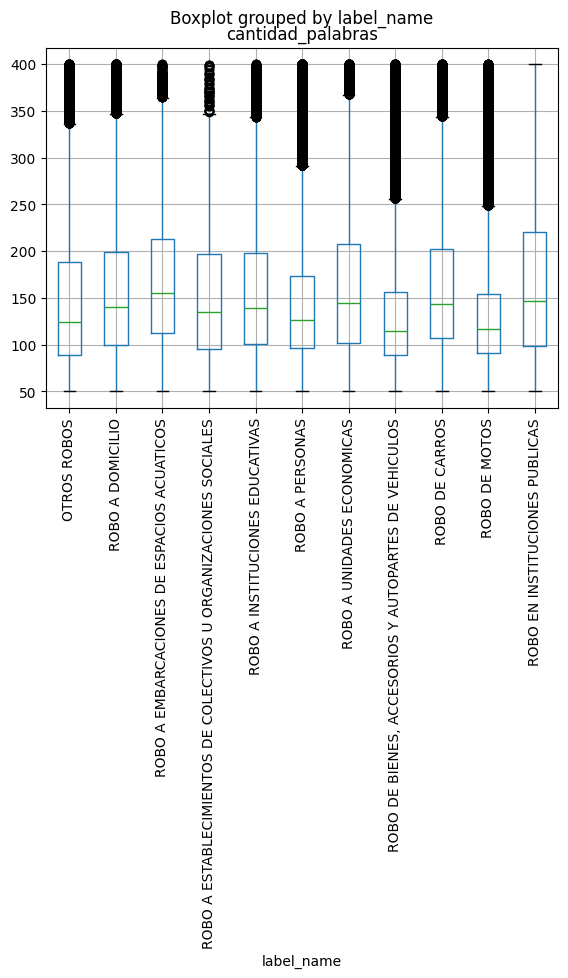
\includegraphics[scale=.8]{imgs/cantidadPalabrasTrainDelitosValidadosBoxPlot.png}
    \caption{Box Plot of Word Count per Validated Crime Categories (e.g., Robo a personas, robo a unidades económicas, etc.)}
    \label{fig:diagramaCajaRelatoTrainValidados}
\end{figure}

Figure \ref{fig:ModelosDelitosValidadosAccxEpoch} shows the
\emph{accuracy} and \emph{loss} as functions of training epochs. It is
observed that there is no overfitting despite the class imbalance.
% ==================== se desactiva porque no es compatible con subfig
% ==================== de la IEEE
% \begin{figure}[h!]
%       \begin{subfigure}[b]{0.8\textwidth}
%         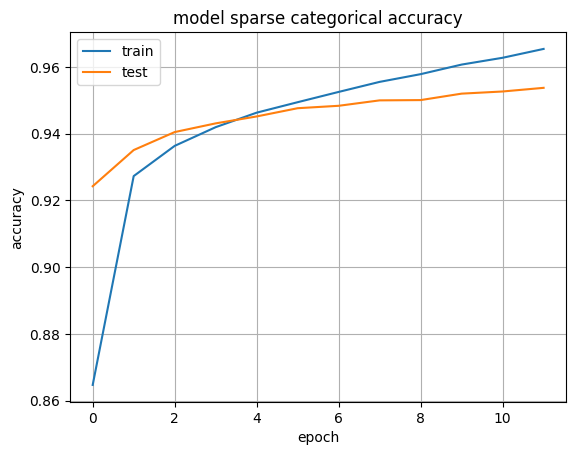
\includegraphics[width=\textwidth]{imgs/DelitosValidadosModeloEntrenamientoAccxEpoch.png} % replace with your first image file
%         \caption{Accuracy por Época}
%       \end{subfigure}
%       \hfill
%       \begin{subfigure}[b]{0.8\textwidth}
%         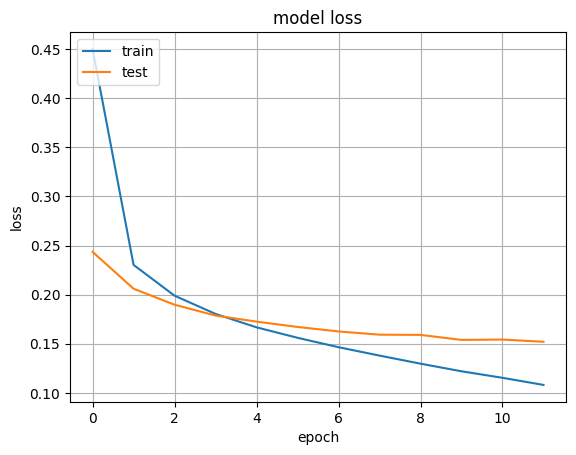
\includegraphics[width=\textwidth]{imgs/DelitosValidadosModeloEntrenamientoLossxEpoch.png} % replace with your second image file
%         \caption{Loss por Época}
%       \end{subfigure}
%       \caption{Accuracy y Loss de entrenamiento y validación}
%       \label{fig:ModelosDelitosValidadosAccxEpoch}
% \end{figure}
% ==================== descomentar si se usa en un contexto diferente
% ==================== a IEEE

\begin{figure}[!t]
    \centering
    \subfloat[Accuracy per Epoch]{%
        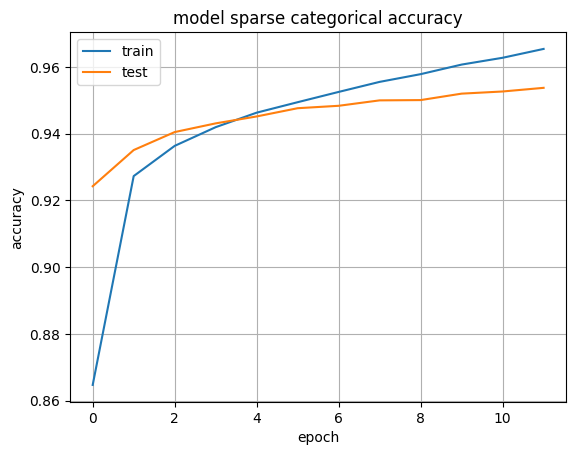
\includegraphics[width=0.8\textwidth]{imgs/DelitosValidadosModeloEntrenamientoAccxEpoch.png}%
        \label{fig:accuracy_epoch}}
    \hfill
    \subfloat[Loss per Epoch]{%
        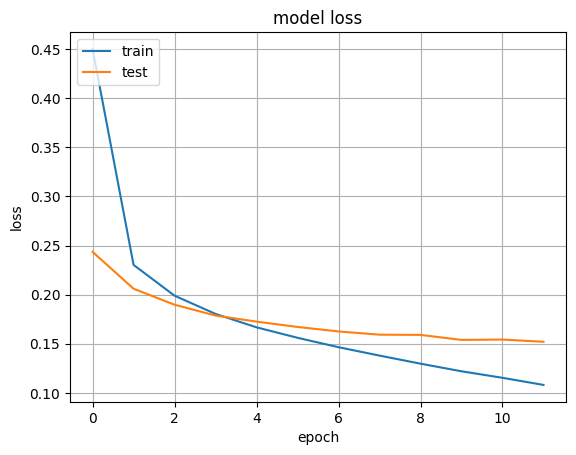
\includegraphics[width=0.8\textwidth]{imgs/DelitosValidadosModeloEntrenamientoLossxEpoch.png}%
        \label{fig:loss_epoch}}
    \caption{Training and Validation Accuracy and Loss}
    \label{fig:ModelosDelitosValidadosAccxEpoch}
\end{figure}


\section{Experimental Results}\label{chap:resultados}

\subsection{Phase 1 Transfer Learning on Basic Taxonomy Dataset Results}
\label{sec:phase-1-dataset-results-tl}

The training results are shown in Figure \ref{fig:loss80} and
\ref{fig:train80} for the optimization function and the performance
metric, respectively. The adjusted model obtained an \emph{accuracy}
of \numprint{0.8248} on the training dataset, \numprint{0.8048} on the
validation dataset, and \numprint{0.8045} on the test dataset.

\begin{figure}[!t]
  \centering
  \subfloat[Loss]{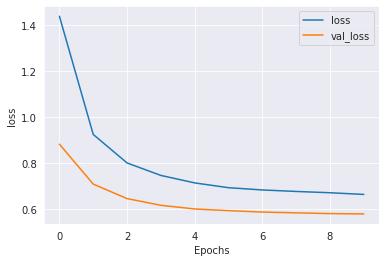
\includegraphics[width=.8\textwidth, height=.5\textheight]{imgs/losstrainacc80.png}
    \label{fig:loss80}}
  \hfil
  \subfloat[Accuracy]{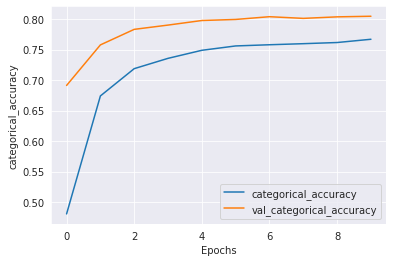
\includegraphics[width=.8\textwidth, height=.5\textheight]{imgs/trainacc80.png}
    \label{fig:train80}}
  \caption{Training of the Machine Learning Text Classification Model}
  \label{fig: results}
\end{figure}

Regarding the $f_1score$ metric, an average of 0.80 was obtained;
where the lowest result is for class 0 with a value of 0.45 and the
highest of 0.87 in class 1. The classifier results on the test dataset
are presented in Table \ref{tab:fscore}, showing the recall and
f-score performance.

\begin{table}[!t]
% increase table row spacing, adjust to taste
\renewcommand{\arraystretch}{1.3}
% if using array.sty, it might be a good idea to tweak the value of
% \extrarowheight as needed to properly center the text within the cells
\caption{Classifier Performance}
\label{tab:fscore}
\centering
% Some packages, such as MDW tools, offer better commands for making tables
% than the plain LaTeX2e tabular which is used here.
\begin{tabular}{ccccc}

\hline
         class &  precision  &  recall & f1-score &  support \\ \hline

           0 &  \numprint{0.58}    &  \numprint{0.36}    &  \numprint{0.45}  &  \numprint{285} \\ 
           1 &   \numprint{0.90}    &  \numprint{0.84}    &  \numprint{0.87}  &  \numprint{457} \\
           2 &   \numprint{0.79}    &  \numprint{0.79}    &  \numprint{0.79}  &  \numprint{613} \\
           3 &   \numprint{0.82}    &  \numprint{0.91}    &  \numprint{0.86}  & \numprint{1666} \\
           4 &   \numprint{0.82}    &  \numprint{0.70}    &  \numprint{0.75}  &  \numprint{328} \\
           5 &   \numprint{0.76}    &  \numprint{0.77}    &  \numprint{0.77}  &  \numprint{651} \\ \hline

   micro avg &     \numprint{0.80} &    \numprint{0.80}   &  \numprint{0.80}  &   \numprint{4000} \\ 
   macro avg &     \numprint{0.78} &    \numprint{0.73}   &  \numprint{0.75}  &   \numprint{4000} \\ \hline
% weighted avg       0.80      0.80      0.80      4000
%  samples avg       0.80      0.80      0.80      4000

\hline
\end{tabular}
\end{table}

\subsection{Phase 2 Fine Tuning on Basic Taxonomy Dataset Results}
\label{sec:phase-2-dataset-results-ft}

The training performance of the FT model in terms of accuracy and loss
metrics is shown in Figures \ref{fig:train92} and \ref{fig:loss92},
respectively. Considering a 10\% threshold for \emph{overfitting}, the
model achieves an accuracy of 90\%. On $d_{train}^T$, the obtained
accuracy is \numprint{0.9922}, while on $d_{valid}^T$, it reaches
\numprint{0.9068}. For $d_{test}^T$, the accuracy is
\numprint{0.9028}. In this context, the FT-trained model improves its
performance by 10\% compared to the TL-trained model, confirming the
hypothesis posited in \textcite{tunstall2022natural}.

However, the performance of a multiclass classifier, such as the one
used for predicting crime labels in this case, cannot rely solely on
\emph{accuracy}. Practice has demonstrated the well-known
\emph{accuracy paradox} \cite{abma2009evaluation}: when
one class dominates the dataset, a poorly performing model tends to
predict the dominant class, introducing errors undetected by this
metric. Therefore, other metrics like \emph{precision}, \emph{recall},
or the confusion matrix are preferred. Table \ref{tab:fscoreModel2}
presents the classification report on the test dataset (i.e., data not
seen during training) using accuracy, precision, and recall.

Finally, Figure \ref{fig:matconfusion} shows the normalized confusion
matrix. The diagonal displays distinctive values corresponding to a
classifier capable of differentiating between multiple classes. The
category with the lowest classification performance is \emph{Robo a
  Unidades Económicas}, achieving 0.79. This means 79 out of 100 cases
are correctly classified. Its primary confusion occurs with \emph{Robo
  a Domicilio} at a value of 0.10 (i.e., 10 out of 100 cases are
misclassified as Robo a Domicilio when they actually belong to Robo a
Unidades Económicas).

% figure* for two column
\begin{figure}[!t]
\centering
\subfloat[Loss]{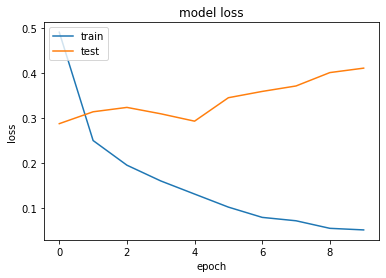
\includegraphics[width=.8\textwidth, height=.5\textheight]{imgs/secondModelLoss.png}
\label{fig:loss92}}
\hfil
\subfloat[Accuracy]{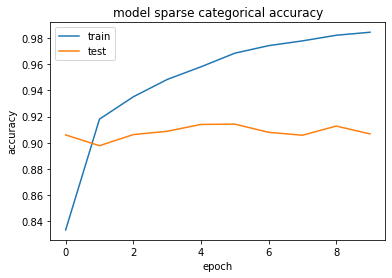
\includegraphics[width=.8\textwidth, height=.5\textheight]{imgs/secondModelFineTuningTrain.png}
\label{fig:train92}}
\caption{Training of the Machine Learning Model for Text Classification in Fine-Tuning Mode}
\label{fig:results}
\end{figure}

\begin{table}[!t]
% increase table row spacing, adjust to taste
\renewcommand{\arraystretch}{1.3}
% if using array.sty, it might be a good idea to tweak the value of
% \extrarowheight as needed to properly center the text within the cells
\caption{FT Classifier Performance}
\label{tab:fscoreModel2}
\centering
% Some packages, such as MDW tools, offer better commands for making tables
% than the plain LaTeX2e tabular which is used here.
\begin{tabular}{ccccc}

\hline
         class &  precision  &  recall & f1-score &  support \\ \hline

           Robo a Unidades Económicas        &  \numprint{0.78}    &  \numprint{0.79}    &  \numprint{0.78}  &  \numprint{297} \\ 
           Robo de Carros                    &   \numprint{0.95}    &  \numprint{0.88}    &  \numprint{0.92}  &  \numprint{363} \\
           Robo de Motos                     &   \numprint{0.95}    &  \numprint{0.93}    &  \numprint{0.94}  &  \numprint{392} \\
           Robo de Bienes, Accesorios y \dots &   \numprint{0.85}    &  \numprint{0.92}    &  \numprint{0.88}  & \numprint{663} \\
           Robo a Domicilio                  &   \numprint{0.87}    &  \numprint{0.89}    &  \numprint{0.88}  &  \numprint{663} \\
           Robo a Personas                   &   \numprint{0.94}    &  \numprint{0.92}    &  \numprint{0.93}  &  \numprint{1671} \\ \hline

          Accuracy                           &     {} &    {}   &  \numprint{0.90}  &   \numprint{4000} \\ 
          Macro Avg                          &     \numprint{0.89} &    \numprint{0.89}   &  \numprint{0.89}  &   \numprint{4000} \\ 
          Weighted Avg                       &   \numprint{0.90}    &  \numprint{0.90} & \numprint{0.90}     & \numprint{4000} \\ \hline
%  samples avg       0.80      0.80      0.80      4000

\hline
\end{tabular}
\end{table}

\begin{figure}[!t]
    \centering
    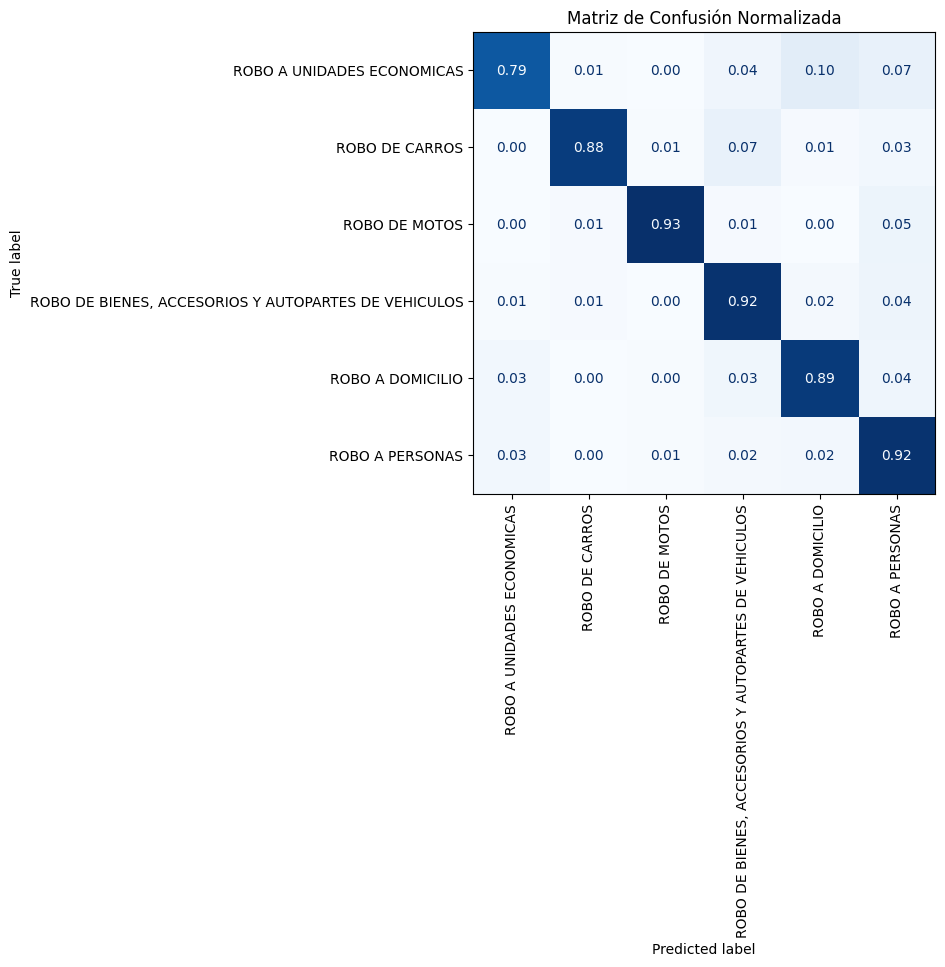
\includegraphics[width=.8\textwidth]{imgs/FineTuning10_epochs.png}
    \caption{Confusion Matrix of the FT Model}
    \label{fig:matconfusion}
  \end{figure}
  
\subsection{Phase 3 Fine Tuning on Extended Taxonomy Dataset Results}
\label{sec:phase-3-extended-dataset-results-ft}

On the test dataset, we compute the performance metrics of the
classifier based on the values of \emph{precision}, \emph{recall},
\emph{accuracy}, and \emph{f1-score}. These results are presented in
Table \ref{tab:reporteClasificacionModeloDelitosValidados}. We also
compute the \emph{normalized confusion matrix}, shown in Figure
\ref{fig:matConfDelitosValidados}.

% \subsubsection{Extended Classifier Report}
\begin{table}[htbp]
    \caption{Performance of the Validated Crimes Classifier}
    \label{tab:reporteClasificacionModeloDelitosValidados}
    \centering
    \scriptsize
    \begin{tabularx}{\textwidth}{p{0.4\textwidth}XXXX}
        \toprule
         & precision & recall & f1-score & support \\
        \midrule
        ROBO A INSTITUCIONES EDUCATIVAS & 0.925995 & 0.946599 & 0.936184 & 1573 \\
        ROBO DE MOTOS & 0.985211 & 0.988317 & 0.986762 & 10785 \\
        ROBO EN INSTITUCIONES PUBLICAS & 0.724528 & 0.474074 & 0.573134 & 405 \\
        ROBO DE CARROS & 0.967669 & 0.980198 & 0.973893 & 7878 \\
        ROBO A ESTABLECIMIENTOS DE COLECTIVOS U ORGANIZACIONES SOCIALES & 0.750000 & 0.752688 & 0.751342 & 279 \\
        ROBO A PERSONAS & 0.969847 & 0.972298 & 0.971071 & 37976 \\
        ROBO A UNIDADES ECONOMICAS & 0.878871 & 0.893877 & 0.886311 & 6794 \\
        ROBO A DOMICILIO & 0.944779 & 0.952335 & 0.948542 & 15504 \\
        ROBO DE BIENES, ACCESORIOS Y AUTOPARTES DE VEHICULOS & 0.977752 & 0.968340 & 0.973023 & 14024 \\
        ROBO A EMBARCACIONES DE ESPACIOS ACUATICOS & 0.965197 & 0.983452 & 0.974239 & 846\\
        OTROS ROBOS & 0.817738 & 0.766006 & 0.791027 & 3936 \\ \hline
        accuracy & {} & {} & 0.954610 & 100000 \\
        macro avg & 0.900690 & 0.879835 & 0.887775 & 100000 \\
        weighted avg & 0.954050 & 0.954610 & 0.954175 & 100000 \\
        \bottomrule
    \end{tabularx}
    
\end{table}
% \subsubsection{Normalized Confusion Matrix}
\begin{figure}
    \centering
    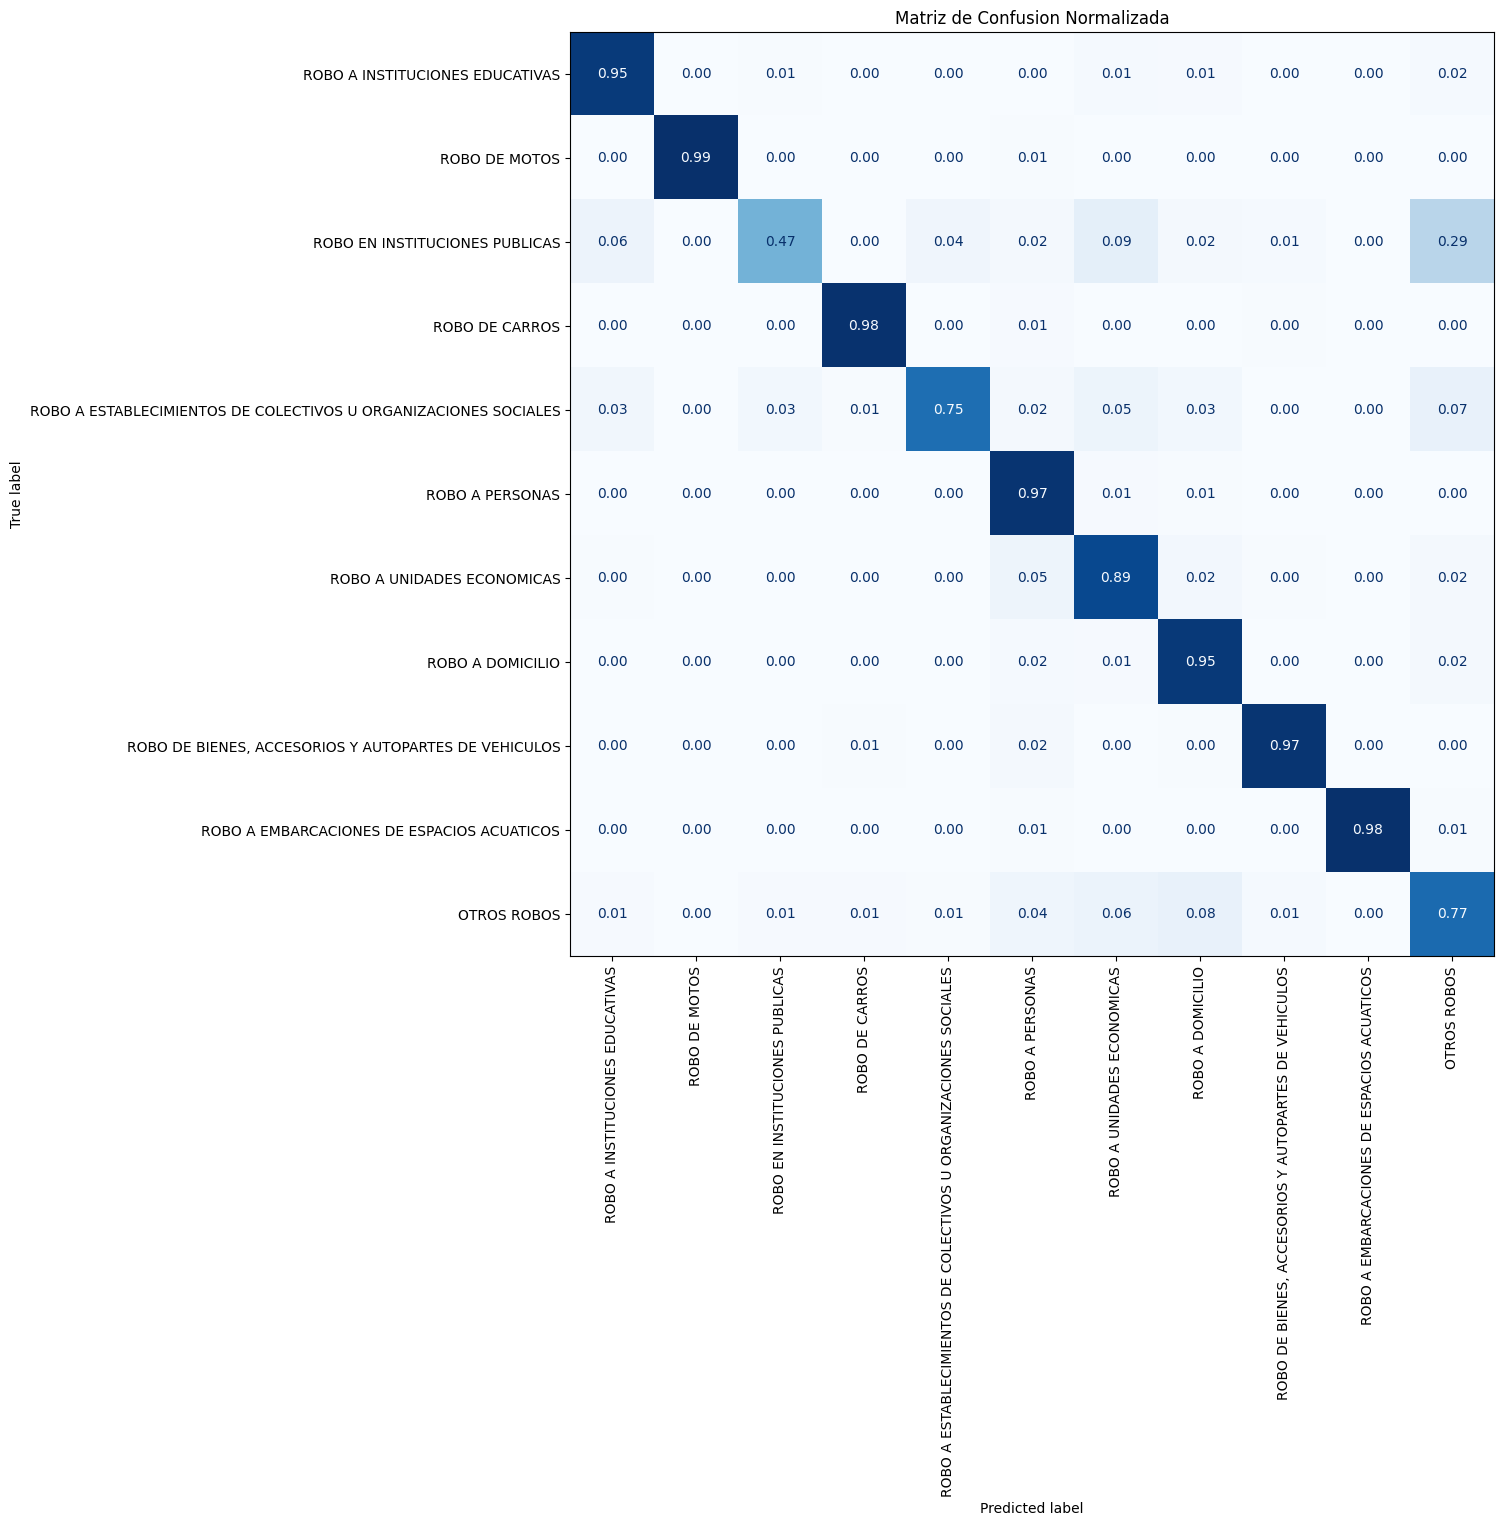
\includegraphics[width=.8\textwidth]{imgs/Matriz de Confusion Normalizada DelitosValidados2.png}
    \caption{Confusion Matrix for the Validated Crimes Model}
    \label{fig:matConfDelitosValidados}
\end{figure}

\section{Conclusions}\label{chap:conclusion}
Transformer-based models have demonstrated enhanced efficacy in
natural language processing tasks, establishing themselves as
state-of-the-art solutions. This study implemented fine-tuning of a
pre-trained model for categorizing robbery narratives into six
distinct classes. Despite class imbalance within the
dataset—particularly the over-representation of \emph{ROBO A
  PERSONAS}—transfer learning from the \modelohuggingface model
yielded sufficient performance to initiate pilot testing for
real-world case predictions. The macro-average f1-score of 80\%
reflects robust classification capability, though class 0 exhibited
comparatively diminished performance.

The integration of fine-tuning techniques improved model accuracy by
10\% relative to baseline approaches, albeit with marginal overfitting
risks attributable to hardware constraints that limited training data
volume ($|d_{\text{train}}^T| < |D_{\text{train}}^T|$). Notably, the
model demonstrated resilience to class imbalance despite the absence
of explicit balancing strategies during training. These findings
underscore the viability of deploying machine learning systems within
legal institutions such as the Fiscalía General del Estado, where
automated narrative classification could optimize resource allocation
and operational workflows. A complementary web application framework
further enables practical model utilization through API integration,
facilitating seamless adoption by legal personnel.

Subsequent model iterations focusing on \emph{delitos validados}
(validated crimes) achieved enhanced precision metrics, attaining
\numprint{0.9546} and surpassing the performance of the \emph{delitos
  seguimiento} (monitored crimes) framework. Computational experiments
confirmed semantic similarity between police reports and SIAF
narratives, while expanded training datasets enabled by TPU
acceleration improved the 11-class classifier's efficacy. Evaluation
metrics—precision, recall, and f1-score—collectively indicate
consistent cross-category performance, with the exception of \say{ROBO
  EN INSTITUCIONES PÚBLICAS} (Theft in Public Institutions) and
\say{ROBO A ESTABLECIMIENTOS DE COLECTIVOS U ORGANIZACIONES SOCIALES}
(Theft in Collective/Social Organizations). These classes, comprising
\numprint{4560} and \numprint{3087} instances respectively, exhibited
lower frequency and predictive performance. Confusion matrix analysis
revealed approximately \numprint{29}\% misclassification between
\say{ROBO EN INSTITUCIONES PÚBLICAS} and \say{OTROS ROBOS} (Other
Thefts), suggesting potential benefits from manual taxonomy refinement
or category consolidation, as evidenced in Table
\ref{tab:GeneracionDataset}.

Collectively, this research affirms the transformative potential of
artificial intelligence in legal domains, where state-of-the-art NLP
models can drive service innovation, task automation, and operational
quality enhancement. Future work should prioritize dataset expansion,
computational resource allocation, and ontological refinements to
address residual classification ambiguities.
% ==================== orginal conclusiones ====================
% Transformer-based models have achieved improved performance in natural
% language processing problems; currently being the state of the art. In
% this article, fine-tuning of a pre-trained model for the
% classification of robbery narratives into 6 categories has been
% carried out.

% The results show that, despite the dataset not being balanced among
% the examples of each class (with the class robo a personas having the
% most examples), the use of \emph{TL} from the pre-trained
% \modelohuggingface model allows obtaining very good performance to
% start pilot tests in the prediction of new cases. The f-score results
% also indicate that, except for the low performance in class 0, an
% average performance of 80\% is obtained.

% As a result of the research, it is concluded that the field of law is
% very suitable for the development of artificial intelligence models,
% which, supported by the state of the art, can generate new services,
% automate tasks, and improve the quality of work carried out in
% strategically important institutions such as the Fiscalía General del
% Estado.

% % phase 2 conclusions
% The use of FT (Fine-Tuning) allowed improving the performance of the
% previous model by 10\%. However, there is a margin close to model
% overfitting. This is a consequence of the model being trained with a
% smaller amount of data due to hardware limitations. The results show
% that the model, although trained on a reduced dataset
% $|d_{train}^T|<|D_{train}^T|$, achieves reasonable results. Indeed,
% the model does not exhibit predictions based on category imbalance; it
% is noted that category balancing has not been performed in any of the
% trainings yet. 

% The possibility of using a machine learning model for natural language
% processing at the Fiscalía General del Estado will optimize time and
% administrative resources. Similarly, the development of a Web
% Application that obtains label predictions by querying the trained
% model, opens the possibility of developing an API for model
% consumption by prosecutor's office staff.

% % Phase 3
% \begin{itemize}
% \item The new model for \emph{delitos validados} (validated crimes)
%   improves precision performance reaching a value of
%   \numprint{0.9546}. Consequently, it outperforms the \emph{delitos
%     seguimiento} (monitored crimes) model.
% \item Computationally, it has been tested with two different
%   techniques, and the police report texts and SIAF narratives are
%   similar.
% \item The improved performance of the \emph{delitos validados} model,
%   which predicts 11 categories, is due to being trained with more
%   examples, enabled by TPU usage.
% \item Among the metrics of \emph{precision}, \emph{recall}, and
%   \emph{f1-score}, adequate classifier performance is observed across
%   categories.
% \item The lowest-performing category is \say{ROBO EN INSTITUCIONES
%     PUBLICAS} (Theft in Public Institutions). As shown in Table
%   \ref{tab:GeneracionDataset}, it has the second-lowest frequency with
%   \numprint{4560} records, followed by \say{ROBO A ESTABLECIMIENTOS DE
%     COLECTIVOS U ORGANIZACIONES SOCIALES} (Theft in Collective/Social
%   Organizations) with \numprint{3087}.
% \item The confusion matrix reveals an approximate \numprint{29}\%
%   confusion between \say{ROBO EN INSTITUCIONES PUBLICAS} and
%   \say{OTROS ROBOS} (Other Thefts). This suggests the need to manually
%   review or merge the \say{OTROS ROBOS} category.
% \end{itemize}
% ==================== original conclusiones ====================
\section{Future Works}\label{chap:futuro}

% As future work, it is proposed to train the model in two scenarios:

% \begin{enumerate}
% \item Training with a data subset $d^T$ with balanced records per
%   class.
% \item Training with the total dataset $D^T$ without class balancing.
% \item Training with the total dataset $D^T$ with class balancing.
% \end{enumerate}

% Additionally, a testing phase will begin for the currently trained
% model, which will be contrasted with the manual classification carried
% out by the Comisión.

Building upon the findings of this study, several avenues for future
research emerge to address current limitations and expand the
practical applicability of the proposed framework. First, dataset
augmentation and/or class-balancing strategies should be prioritized to
mitigate performance disparities among underrepresented categories
such as \say{ROBO EN INSTITUCIONES PÚBLICAS}. Synthetic data
generation or targeted data collection could alleviate biases induced
by imbalanced training samples, potentially reducing the observed
\numprint{29}\% misclassification rate between semantically adjacent
categories. Additionally, expanding computational resources to
leverage full-scale datasets ($|D_{\text{train}}^T|$) rather than
subsets ($|d_{\text{train}}^T|$) would enable more robust model
training, minimizing overfitting risks while improving
generalizability.

From an operational perspective, deploying the developed web
application in controlled pilot environments at the Fiscalía General
del Estado would validate its real-world efficacy and user
acceptance. As a matter of fact, current model is being used by
\textit{Departamento de Estadística y Sistemas de Información} at
Fiscalía General del Estado. It helps to predict robbery categories
using the registered narratives. However, extending its use to other
departments could be studied. Moreover, longitudinal studies assessing the
model’s performance drift over time could inform maintenance protocols
for periodic retraining. Furthermore, extending the taxonomy to
encompass broader criminal typologies or interlinked legal processes
(e.g., sentencing recommendations or case prioritization) would
amplify the system’s utility. Collaborative efforts with legal experts
to refine category definitions and annotation guidelines are essential
to ensure algorithmic fairness and jurisdictional compliance,
particularly in high-stakes decision-making contexts.

A promising direction for future work involves the development of an
abstractive transformer-based question-answering (QA) model to enhance
case analysis by retrieving and synthesizing relevant details from
robbery narratives. Such a model could assist legal practitioners by
automatically extracting key facts (e.g., modus operandi, stolen
items, or suspect descriptions) from unstructured reports, thereby
improving efficiency in case review and evidence
compilation. Leveraging architectures like BERT \cite{devlin2018bert}
or T5 \cite{raffel2023T5} could enable the system to generate concise,
context-aware summaries while preserving factual accuracy—a critical
requirement in legal applications. As a matter of fact, we present a
preliminary work on the mater of Question Answering from robbery
narratives stating potential outcomes in Section
\ref{sec:an-abstr-qa-model}.

Finally, ethical and
transparency considerations warrant dedicated investigation, including
the development of explainability interfaces to demystify model
predictions for legal practitioners. Establishing audit frameworks to
monitor algorithmic biases and performance disparities across
demographic or geographic variables will be critical for maintaining
public trust in AI-driven judicial tools. These interdisciplinary
efforts would position such systems not merely as technical artifacts,
but as scalable, accountable solutions for modernizing legal
workflows.

\subsection{An Abstractive Question Answering Model}
\label{sec:an-abstr-qa-model}

Extractive question answering (QA) systems hold significant potential
for automating information retrieval in specialized domains such as
legal and criminal justice. While transformer-based models (e.g., BERT
and its variants) have shown strong performance in general NLP tasks,
their adaptation to domain-specific contexts—particularly legal
document analysis—remains an open challenge requiring further
investigation. In criminal justice systems, efficient extraction of
structured information from unstructured crime reports could
significantly improve case handling, resource allocation, and
decision-making processes. This exploratory work will focus on robbery
cases processed by the Fiscalía General del Estado in Ecuador, where
the high volume of reports and the complexity of legal language
present substantial barriers to manual analysis. By leveraging and
fine-tuning transformer-based models, we aim to assess their
effectiveness in enhancing information retrieval from legal texts. If
successful, this approach could support legal practitioners by
reducing processing time and improving accuracy, ultimately
contributing to more efficient judicial workflows and better public
service delivery. Future research will involve dataset curation, model
adaptation, and rigorous evaluation to determine the feasibility and
limitations of this application.

\subsubsection{An Introduction to Legal Question Answering}
\label{sec:an-intr-legal-qa-paper}

Transformer models have emerged as powerful tools in natural language
processing, enabling more accurate and efficient extraction of
relevant information from complex texts such as criminal
reports. These models utilize self-attention mechanisms to weigh the
importance of different words in a sentence, allowing for better
context understanding and improved performance in tasks like question
answering. By fine-tuning these models on domain-specific datasets,
researchers can enhance their ability to discern pertinent details and
provide precise answers to inquiries related to criminal incidents.

The implementation of extractive question answering systems in legal
contexts not only enhances the efficiency of information retrieval but
also addresses challenges related to data variability and complexity
inherent in criminal reports. As these models are fine-tuned on
diverse datasets, they can improve their generalizability across
different types of legal documents, ensuring that critical details are
accurately captured regardless of nuances in language or structure
\cite{jha2022extractive}. Moreover, recent advancements in model
architectures, such as the integration of dynamic masking techniques,
have shown promise in further refining performance by enabling models
to better adapt to varying levels of difficulty in questions posed
about complex narratives \cite{Pearce_Zhan_Komanduri_Zhan_2021}. This
evolution highlights the potential for transformer-based models to
facilitate more informed decision-making processes within the justice
system, ultimately contributing to enhanced outcomes for legal
practitioners and stakeholders alike.

The Fiscalía General del Estado, which is the Prosecutor’s Office in
Ecuador, handles cases ranging from criminal investigations to public
safety concerns, aiming to uphold justice and protect the rights of
citizens. In this context, crimes of robbery are highly prevalent and
present significant challenges for law enforcement
agencies. Understanding the patterns and motivations behind these
crimes can lead to more effective prevention strategies and better
resource allocation, ultimately fostering a safer community for all
citizens. Additionally, it is important to analyze all the information
gathered through crime reports. Many users also rely on this
information to access insurance coverage for items lost during theft
(e.g., cell phones, computers, automobiles, automobile parts,
etc.). The volume of cases that need to be reviewed by prosecutors is
substantial. Consequently, it is of interest to explore the use of
artificial intelligence in designing and training models that can help
reduce the high demand and improve public service.

\subsubsection{Legal Question Answering Related Works}
\label{sec:legal-quest-answ-literature}

There is a significant interest within both the scientific community
and legal institutions in studying the applications of AI in this
expansive field. The current state of the art in Natural Language
Processing (NLP) with Deep Learning (DL) primarily focuses on the use
of transformer-based architectures, which have demonstrated superior
performance across various NLP tasks.

In \cite{Vold_Conrad_2021} the deployment of a RoBERTa Base
question-answer classification model specifically for legal questions
is discussed.  It compares the performance of this transformer model
against a traditional linear SVM in the legal domain, using the
PRIVACYQA dataset. The results indicate that RoBERTa significantly
outperforms the SVM, achieving a 31\% improvement in F1-score and a 41\%
improvement in Mean Reciprocal Rank, demonstrating the effectiveness
of transformers in enhancing answer retrieval for legal inquiries. In
\cite{Shao_Guo_Chen_Zepeng_2019}, the researchers focus on a
Transformer-based neural network for answer selection in general
question answering (QA) systems, not specifically in the legal
domain. While Transformers are effective in extracting global
information and improving answer selection, the research does not
address their application in law-related question answering. For
insights on using Transformers in legal contexts, further research
specific to legal NLP applications would be necessary. For information
retrieval, \cite{Kim_Rabelo_Babiker_Rahman_Goebel_2024} discuss the
use of transformer-based approaches for legal information retrieval
and entailment, specifically in the context of the COLIEE
competition. For case law retrieval (Task 1), a sentence-transformer
model was employed to create numeric representations of case
paragraphs, facilitating similarity assessments. In entailment (Task
4), a fine-tuned DeBERTa large language model was utilized, achieving
third place among eight teams. These methods demonstrate the
effectiveness of transformers in addressing legal question answering
challenges. Another area of interest is to predict legal judgments. In
\cite{Gosh_Kumar_2024} six transformer-based models (BERT, XLNet,
RoBERTa, DeBERTa, ELECTRA, and BigBird) are evaluated in predicting
legal judgments using the ILDC dataset. It highlights the potential of
these models in automating legal decision-making, with newer models
achieving up to 80\% accuracy compared to 76\% for older models. This
comparative analysis underscores the advancements in NLP technology
and its applicability in the legal domain, suggesting a promising
future for question answering in law through transformer
models. Finally, in \cite{Peric_Mijic_Stammbach_Ash_2020} the use of
transformers to generate legal text is addressed, indicating their
potential to assist in legal practice. The findings suggest that these
models can effectively generate judicial opinions and help
differentiate between human and machine-generated legal texts, which
could be beneficial for tasks like drafting contracts and briefs,
although direct application to question answering is not discussed.

\subsubsection{Robbery Model for LQA}
\label{sec:robbery-model-lqa}

In order to address LQA, we propose a specialized question-answering
model based on the architecture of
mrm8488/bert-base-spanish-wwm-cased-finetuned-spa-squad2-es. The model
needs to be adapted for legal domain applications, specifically those
of the Fiscalía General del Estado in processing robbery case
documentation. The implementation methodology will be structured as
follows:

\begin{enumerate}
    \item \textbf{Dataset Preparation}: Curating and annotating domain-specific legal documents to construct a robust training corpus.
    \item \textbf{Prompt Engineering}: Designing optimized query formulations to enhance model performance on legal text comprehension tasks.
    \item \textbf{Dataset Preprocessing}: Implementing text normalization and feature extraction pipelines tailored for legal domain data.
    \item \textbf{Model Fine-tuning}: Adapting the pre-trained architecture through domain-specific optimization techniques.
    \end{enumerate}

\paragraph{Dataset Preparation with aid of Generative AI}

To prepare the dataset for this task, Generative Artificial
Intelligence (GAI) will be employed to extract answers for a
predefined set of common questions in robbery cases. The proposed
model for this purpose is
\texttt{meta-llama/Meta-Llama-3-8B-Instruct}. An initial analysis of
word count distribution per crime report will be conducted to
establish quality thresholds. Preliminary observations suggest a mean
length of 112 words, with an expected range between 82 and 150
words. Reports falling outside this range will be excluded as
potential outliers. Consequently, the final dataset will comprise only
those crime reports \(w\) where the word count \(\Gamma(w)\) satisfies
\(82 \leq \Gamma(w) \leq 150\). The original dataset contains 174,594
samples, which will serve as the foundation for this filtering
process.

A LLM would be used to generate responses for a predefined set of
common questions (Table \ref{tab:org640ecfb}). The LLM is configured
to operate as a specialized data science assistant with the objective
of creating a Spanish-language dataset formatted according to the
SQuAD (Stanford Question Answering Dataset) framework. The
implementation involves providing the LLM with two key inputs: (1) the
full text of the crime report serving as the \texttt{context}, and (2)
individual questions from Table \ref{tab:org640ecfb} as the
\texttt{question} component. The model is specifically instructed to
return its output in JSON format, containing the following fields:
\texttt{context}, \texttt{question}, \texttt{answer\_text},
\texttt{answer\_start}, \texttt{answer\_end}, and
\texttt{impossible\_find\_answer}.

The span indices (\texttt{answer\_start} and \texttt{answer\_end}) are
automatically derived by locating the \texttt{answer\_text} within the
provided context. In instances where the system either cannot identify
a valid answer or fails to generate an appropriate response, the
boolean flag \texttt{impossible\_find\_answer} is set to
\texttt{True}, providing a mechanism for tracking unsuccessful
extraction attempts. This approach facilitates both answer validation
and subsequent analysis of model performance.

\begin{table}[htbp]
\caption{\label{tab:org640ecfb}Common questions}
\centering
\begin{tabular}{l}
\hline
Question\\
\hline
¿Qué objetos fueron robados?\\
¿En qué fecha ocurrió el incidente?\\
¿A qué hora sucedió el robo?\\
¿En qué dirección o entre qué calles sucedió el robo, suceso incidente?\\
¿Qué valor en dólares tenían los objetos sustraídos o robados?\\
\hline
\end{tabular}
\end{table}

After conducting preliminary experiments using the Hugging Face
Inference Client, we estimate that 1,544 samples would take over a
4-hour period to be processed; representing approximately 1\% of the
complete dataset. Initial analysis of the results revealed two notable
limitations: (1) instances where the LLM may fail to generate
appropriate responses, and (2) cases where the model produced
irrelevant content. These observations highlight the necessity for
implementing a manual verification protocol to ensure data
quality. Future work will focus on optimizing the processing
pipeline to improve both efficiency and output reliability.

\paragraph{LQA Model Fine Tuning}

Here, we outline the methodological framework to be employed for
training a question-answering model designed to process robbery
reports from Ecuador's Fiscalía General del Estado. The procedure may
consist of of the following key steps:

\begin{itemize}
\item \textbf{Dataset Train and Test split:} An initial dataset to
  analyze model's capabilities would be of 4572 samples, according to
  our expected results from our research. the dataset was divided into
  training and testing sets, with 20\% of the cases allocated for
  performance evaluation. Table \ref{tab:org06f9053} displays the
  number of samples in each set.
\item \textbf{Pre-trained Model Loading:}The
  \texttt{mrm8488/bert-base-spanish-wwm-cased-finetuned-spa-squad2-es}
  model was selected for fine-tuning due to its specialized
  architecture for Spanish language processing and demonstrated
  effectiveness in QA tasks. This selection was further justified by
  preliminary evaluations conducted on the base model, which achieved
  an F1-score of 81.70 without additional training, indicating strong
  baseline performance for the target application.
\item \textbf{Preprocessing:}To fine-tune the model, both the question
  and the answer must undergo tokenization and embedding
  representation. Following this process, the indices marking the
  start and end positions of the answer require recalibration based on
  the tokenized embeddings. For lengthy textual contexts, truncation
  is selectively applied to the context segment, while a sliding
  window of 128 tokens is implemented to preserve answer integrity
  during truncation. Although the majority of samples in the current
  dataset contain contexts with fewer than 100 words—rendering this
  scenario improbable—the methodology has been systematically
  incorporated into the implementation as a precautionary
  measure. This approach ensures robustness while maintaining
  computational efficiency during model training.
\item \textbf{Evaluation Metrics:}The evaluation framework will employ
  the \texttt{squad\_v2} benchmark metrics, which incorporate both
  F1-score and exact match measurements. These metrics will be
  implemented through a custom evaluation function compatible with the
  Hugging Face Trainer class, allowing for standardized performance
  assessment during model development.
\item \textbf{Training Protocol:} The training regimen will utilize
  the hyperparameters specified in Table \ref{tab:org4204959}, with
  particular emphasis on employing a conservative learning rate. This
  approach aligns with established fine-tuning best practices, as it
  preserves the pre-trained model's knowledge while facilitating
  domain adaptation. Preliminary results suggest that domain-specific
  fine-tuning yields marginal improvements over the base model's
  performance, though this observation may be partially attributable
  to dataset size constraints in the current experimental
  setup. Further investigation with complete datasets will be
  necessary to fully validate these findings.
\end{itemize}


\begin{table}[htbp]
\caption{\label{tab:org06f9053}Dataset Train and Test Split}
\centering
\begin{tabular}{lr}
Partition & \# Samples\\
\hline
Train & 3657\\
Test & 915\\
Total & 4572\\
\end{tabular}
\end{table}


\begin{table}[htbp]
\caption{\label{tab:org4204959}Training Parameters}
\centering
\begin{tabular}{ll}
Parameter & Value2\\
\hline
Strategy & epoch\\
Learning rate & \(2 \times 10^{-5}\)\\
batch & 64\\
epochs & 10\\
weight decay & 0.01\\
fp16 & True\\
metric for best model & F1 (eval)\\
\end{tabular}
\end{table}

\paragraph{Expected Results}

This study is expected to demonstrate measurable improvements in model
performance through domain-specific fine-tuning. The evaluation will
compare two key metrics:

\begin{enumerate}
\item Baseline performance using the pre-trained model
\item Anticipated performance after
fine-tuning
\end{enumerate}

Based on preliminary experiments and similar studies in the
literature, we project that the fine-tuned model will achieve:

\begin{itemize}
\item An F1-score improvement of approximately 1-3 percentage points
  over the baseline
\item A target F1-score of 82-84 on the evaluation dataset
\item Enhanced exact match accuracy for domain-specific terminology
\end{itemize}

The performance gains are expected to be particularly noticeable for:
\begin{itemize}
\item Questions involving legal terminology specific to robbery cases
\item Longer, more complex narratives that benefit from domain adaptation
\item Low-frequency answer types that require specialized knowledge
\end{itemize}

These projected improvements will be validated through comprehensive
testing once the full dataset processing is complete. The final
evaluation will include both quantitative metrics and qualitative
analysis of answer quality.





\section*{Acknowledgments}

The authors wish to thank the Fiscalía General del Estado for allowing
research in the development of machine learning models for natural
language processing problems applied to tasks specific to the
institution. Thanks are also due to the Dirección de Estadística y
Sistemas de información for generating the dataset used in this
research.

% Can use something like this to put references on a page
% by themselves when using endfloat and the captionsoff option.
\ifCLASSOPTIONcaptionsoff
  \newpage
\fi



% trigger a \newpage just before the given reference
% number - used to balance the columns on the last page
% adjust value as needed - may need to be readjusted if
% the document is modified later
%\IEEEtriggeratref{8}
% The "triggered" command can be changed if desired:
%\IEEEtriggercmd{\enlargethispage{-5in}}

% references section

% can use a bibliography generated by BibTeX as a .bbl file
% BibTeX documentation can be easily obtained at:
% http://mirror.ctan.org/biblio/bibtex/contrib/doc/
% The IEEEtran BibTeX style support page is at:
% http://www.michaelshell.org/tex/ieeetran/bibtex/
%\bibliographystyle{IEEEtran}
% argument is your BibTeX string definitions and bibliography database(s)
%\bibliography{IEEEabrv,../bib/paper}
%
% <OR> manually copy in the resultant .bbl file
% set second argument of \begin to the number of references
% (used to reserve space for the reference number labels box)

% \begin{thebibliography}{1}

% \bibitem{IEEEhowto:kopka}
% H.~Kopka and P.~W. Daly, \emph{A Guide to \LaTeX}, 3rd~ed.\hskip 1em plus
%   0.5em minus 0.4em\relax Harlow, England: Addison-Wesley, 1999.

% \end{thebibliography}

% \bibliography{./bibtex/mybib.bib}
\printbibliography

% biography section
% 
% If you have an EPS/PDF photo (graphicx package needed) extra braces are
% needed around the contents of the optional argument to biography to prevent
% the LaTeX parser from getting confused when it sees the complicated
% \includegraphics command within an optional argument. (You could create
% your own custom macro containing the \includegraphics command to make things
% simpler here.)
%\begin{IEEEbiography}[{\includegraphics[width=1in,height=1.25in,clip,keepaspectratio]{mshell}}]{Michael Shell}
% or if you just want to reserve a space for a photo:

% ======== bibiografía =============
% \begin{IEEEbiography}{Michael Shell}
% Biography text here.
% \end{IEEEbiography}

% % if you will not have a photo at all:
% \begin{IEEEbiographynophoto}{John Doe}
% Biography text here.
% \end{IEEEbiographynophoto}

% % insert where needed to balance the two columns on the last page with
% % biographies
% %\newpage

% \begin{IEEEbiographynophoto}{Jane Doe}
% Biography text here.
% \end{IEEEbiographynophoto}

% You can push biographies down or up by placing
% a \vfill before or after them. The appropriate
% use of \vfill depends on what kind of text is
% on the last page and whether or not the columns
% are being equalized.

%\vfill

% Can be used to pull up biographies so that the bottom of the last one
% is flush with the other column.
%\enlargethispage{-5in}



% that's all folks
\end{document}

%%% Local Variables:
%%% mode: LaTeX
%%% TeX-master: t
%%% End:
